\documentclass[ %
fleqn, % left aligned equations.
11pt, % normal textsize.
oneside, % single side page, use twoside if >50 pages.
print=false, % sets all link colors to black and redefines colors in greyscale (lower printing costs).
language=english, % use only ngerman or english.
thesis=true, % set to false when writing a report
]{CMSthesis}

%======================== please fill in your data here ==========================
\SetType{Master of Science (M.Sc.)} % Bachelor, Master.
\SetFieldOfStudy{Information Technologies for the Built Environment} % TODO: check official program name
% The class typesets the title with \nohyphens (hyphenation off). Justified
% setting would therefore have to stretch the word spaces and can overrun the
% margin, so the title is set ragged right: LaTeX breaks the lines by itself and
% no manual \\ is needed. Keep the leading \raggedright and the closing
% \endgraf (\SetTopic takes a short argument, so a literal \par breaks it).
\SetTopic{\raggedright Evaluating Methods for Building Attribute Prediction from Street View Imagery in Archetype-Based Building Stock Enrichment\endgraf} % Topic of your thesis
% \SetSubtopic{TODO: subtitle if any} % Remove otherwise
\SetAuthor{Pei-Ling Song} % comma separated list for report
\SetMatrikulationNo{03798081} % only for thesis
\SetEmail{peiling.song@gmail.com} % only for thesis
\SetZipCode{80333} % only for thesis
\SetLocation{München} % only for thesis
\SetStreet{Arcisstrasse 21} % only for thesis

\SetStart{} % Date of registration; not printed on the thesis title page
\SetEnd{September 16, 2026} % Date of submission

%======================== Add supervisors ===========================
% \SetReferent{} and \SetReferentAffil{} add a separate "Referent" (examining
% professor) block above the supervisors. Left unset for now.
\AddSupervisor{Prof. Dr.-Ing. André Borrmann, Agata Dalach, Jose Quesada Allerhand} % comma separated list, one line each
\AddAffil{\DAchair} % Add affiliation of the supervisors, deactivated for report

%======================== load extra packages here ===============================
% \usepackage{...package name...}

%======================== Silbentrennung =========================================
\hyphenation{Sil-ben-tren-nung pa-ra-me-tri-schen}

%======================== Programmiersprachen ====================================
\input{codestyles}

%======================== Settings ===============================================
% \setcounter{secnumdepth}{3} % use this if you want to increase toc depth.
%\DefineColor[0.5]{kwcolor}{default}{Green}

%======================== References and Abbreviations ===========================
\addbibresource{./literature/references.bib}

\makeglossaries
% Usage in text:
% \ac{<label>}   Full form (long (short)) on first use, short form afterwards.
% \acs{<label>}  Short form only.
% \acf{<label>}  Always the full form.
% \acl{<label>}  Long form only.
% Plural: append "p", e.g. \acp{VLM}. Capitalised: \Ac, \Acs, \Acf, \Acl.
%
% Long forms are stored in lower case to ensure that \ac{} reads correctly inside a
% sentence; use \Ac{} at the beginning of a sentence. Only abbreviations that
% are actually used in the text appear in the List of Abbreviations.
%
% Use {} brackets if a value contains special characters or a comma!

\newabbreviation{AoV}{AoV}{angle of view}

\newabbreviation{BAG}{BAG}{Basisregistratie Adressen en Gebouwen}

\newabbreviation{CNN}{CNN}{convolutional neural network}

\newabbreviation{CV}{CV}{computer vision}

\newabbreviation{EPC}{EPC}{Energy Performance Certificate}

\newabbreviation{LightGBM}{LightGBM}{Light Gradient Boosting Machine}

\newabbreviation{LoD}{LoD}{Level of Detail}

\newabbreviation{ML}{ML}{machine learning}

\newabbreviation{MLP}{MLP}{multilayer perceptron}

\newabbreviation{OSM}{OSM}{OpenStreetMap}

\newabbreviation{SVI}{SVI}{street view imagery}

\newabbreviation{TABULA}{TABULA}{Typology Approach for Building Stock Energy Assessment}

\newabbreviation{UBEM}{UBEM}{urban building energy modelling}

\newabbreviation{ViT}{ViT}{Vision Transformer}

\newabbreviation{VLM}{VLM}{vision-language model}
 % Definition der Abkürzungen (Abbreviations)
\input{content/00d_symbollist} % not implemented yet
%\input{content/00e_glossary}

%=================================================================================
\begin{document}
\pagestyle{empty}
\pagenumbering{Alph}
%========== Titelseite, Zusammenfassung, Inhaltsverzeichnis, etc. ================
\maketitle
\pagenumbering{Roman}
\cleardoublepage

\section*{Abstract}

Large-scale archetype-based urban building energy modelling relies on building attributes that are often incomplete or missing from open geospatial datasets. This study evaluates whether building type, construction year, and floor count predicted from street view imagery (SVI) can replace reference building attributes from administrative records and reconstructed 3D data in a TABULA-NL building stock enrichment workflow. The experimental dataset comprises 47,150 images linked to 10,086 residential buildings in four Dutch study areas. Three vision configurations were evaluated: a ResNet-50 fine-tuned across all layers, a frozen DINOv2 backbone with supervised prediction heads, and InternVL3-2B without parameter updating. Evaluation spanned building attribute prediction, TABULA-NL archetype assignment, physically weighted differences from reference archetypes, and energy class prediction under a controlled change from reference to predicted attributes.

DINOv2 performed best on six of seven attribute metrics, including a mean absolute error of 9.40 years for construction year. Its joint cell accuracy exceeded both the uniform random expectation and the majority cell baseline. Holding the reconstructed building areas and window-to-wall ratios constant, the aggregate transmission heat transfer coefficient calculated from its predicted archetype cells was approximately 10\% higher than that calculated from reference cells. Replacing reference attributes with DINOv2 predictions had little effect on binary macro F1. However, both the reference attribute condition and the predicted attribute condition had low recall for classes D to G. Direct image classification achieved the highest binary macro F1.

The findings support the conditional use of building attributes predicted from SVI when reference building attributes are unavailable. Suitability depends on the attribute, subsequent task, dataset composition, and geographic relationship between training and application data.

\newpage
\section*{Zusammenfassung}

Großmaßstäbliche urbane Gebäudeenergiemodelle auf Basis von Archetypen benötigen Gebäudeattribute, die in offenen Geodaten häufig unvollständig sind oder fehlen. Diese Arbeit untersucht, ob aus Straßenbildaufnahmen (SVI) vorhergesagte Angaben zu Gebäudetyp, Baujahr und Geschosszahl die Referenzattribute aus Verwaltungsregistern und rekonstruierten dreidimensionalen Daten in einem Verfahren zur Anreicherung des Gebäudebestands mit Archetypen aus TABULA-NL ersetzen können. Der experimentelle Datensatz umfasst 47.150 Bilder, die mit 10.086 Wohngebäuden in vier niederländischen Untersuchungsgebieten verknüpft sind. Bewertet wurden ein in allen Schichten nachtrainiertes ResNet-50, DINOv2 mit eingefrorenen Gewichten und überwachten Vorhersageköpfen sowie InternVL3-2B ohne zusätzliches Training. Die Bewertung umfasste die Vorhersage von Gebäudeattributen, die Zuweisung von Archetypen aus TABULA-NL, physikalisch gewichtete Abweichungen von den Referenzarchetypen und die Klassifikation von Energieklassen unter kontrollierter Ersetzung einzelner Attribute.

DINOv2 erzielte bei sechs von sieben Attributmetriken das beste Ergebnis. Der mittlere absolute Fehler für das Baujahr betrug 9,40 Jahre. Die Genauigkeit der gemeinsamen Archetypzelle übertraf sowohl den Erwartungswert einer gleichverteilten Zufallszuweisung als auch die Baseline der häufigsten Zelle. Bei konstant gehaltenen rekonstruierten Gebäudeflächen und Verhältnissen von Fensterfläche zu Wandfläche war der aus den vorhergesagten Archetypzellen berechnete aggregierte Transmissionskoeffizient etwa 10\% höher als der aus den Referenzzellen berechnete Wert. Die Ersetzung der Referenzattribute durch Vorhersagen von DINOv2 veränderte den binären Makro F1 nur geringfügig. Sowohl die Bedingung mit Referenzattributen als auch die Bedingung mit vorhergesagten Attributen erzielten jedoch eine geringe Sensitivität für die Klassen D bis G. Die direkte Bildklassifikation erreichte beim binären Makro F1 den höchsten Wert.

Die Ergebnisse stützen den bedingten Einsatz von aus Straßenbildaufnahmen abgeleiteten Attributen, wenn keine Referenzdaten verfügbar sind. Die Eignung hängt vom betrachteten Attribut, von der nachgelagerten Aufgabe, von der Zusammensetzung der Stichprobe und von der geografischen Beziehung zwischen den Trainingsdaten und dem Anwendungsgebiet ab.
 % not needed in report

\tableofcontents % Inhaltsverzeichnis
\cleardoublepage

%========== Optionale Verzeichnisse, nur nach Abstimmung mit Betreuer ============
\listoffigures % List of Figures, optional
\cleardoublepage

\listoftables % List of Tables, optional
\cleardoublepage

% \lstlistoflistings % Algorithmusverzeichnis, optional
% \cleardoublepage
% \glsaddall
\printglossary[type=abbreviations,style=super,title={List of Abbreviations}] % only abbreviations used in the text are listed, optional
% \printglossary[type=symbols,style=super4col,title={List of Symbols}]   % list of symbols, optional — enable if symbols are used
\cleardoublepage

%============ Ab hier der eigentliche Inhalt der Master Thesis ===================
\parskip 8pt % Abstand zwischen aufeinanderfolgenden Absätzen
\pagenumbering{arabic} % 

\chapter{Introduction}
\label{ch:introduction}

\section{Background}
\label{sec:background}

The building stock represents a major source of global energy demand and a central target of climate policy. Within the energy demand of buildings, residential buildings account for 70\%, while commercial and public buildings account for the remaining 30\% \parencite{iea2025}. In the European Union, buildings account for approximately 40\% of final energy consumption and 36\% of energy-related greenhouse gas emissions \parencite{epbd2024}. These magnitudes make reductions in the energy demand and emissions of existing buildings central to European climate policy. Accordingly, the 2024 recast of the Energy Performance of Buildings Directive establishes the objective of achieving a zero-emission building stock by 2050 \parencite{epbd2024}. Achieving this objective requires reliable information on the existing building stock to support large-scale energy-performance assessment and the prioritisation of renovation measures \parencite{hettinga2023}. The policy challenge therefore translates into an information challenge at the scale of the existing building stock.

\Ac{UBEM} provides a way to assess this performance at the scale of groups of buildings. \ac{UBEM} applies physical models of heat and mass flows in and around buildings to predict operational energy use and indoor and outdoor environmental conditions \parencite{reinhart2016}. As shown in Figure~\ref{fig:ubem_workflow}, a basic \ac{UBEM} workflow combines climate data, building geometry, construction standards, and usage schedules as inputs to simulations of energy use and environmental performance. Although detailed inputs can be collected for individual buildings or small samples, collecting them consistently across larger urban areas is resource intensive and often impractical \parencite{reinhart2016}. The scalability of \ac{UBEM} therefore depends on representing the building stock with information that can be obtained consistently at urban scale.

\begin{figure}[htbp]
	\centering
	\includegraphics[width=\textwidth]{figures/fig/fig_3_1_UBEM_workflow}
	\caption{General workflow for urban building energy modelling. Geometry, building attributes, and archetype information provide inputs for simulation. The results support assessments of energy use, carbon emissions, and energy performance. Based on \textcite{ang2020}.}
	\label{fig:ubem_workflow}
\end{figure}

Building archetypes address this scalability constraint by representing groups of buildings with similar physical and operational characteristics \parencite{reinhart2016,shen_archetype_2024}. They are used extensively in national and regional bottom-up building stock models. Archetype generation consists of two complementary steps: segmentation and characterisation. Segmentation divides the building stock into groups according to characteristics such as building shape, age, use, climate, and technical systems. Characterisation then assigns each archetype a complete set of thermal and operational properties, including construction assemblies, usage patterns, and building systems \parencite{reinhart2016}. Depending on the application scale and selected segmentation parameters, one archetype may represent fewer than 50 or as many as 500,000 buildings \parencite{reinhart2016}. Archetypes therefore reduce building-specific input requirements, but their usefulness depends on assigning each building to an appropriate group.

European building typologies operationalise this grouping process at national, regional, and municipal scales \parencite{loga2016}. Among them, the \ac{TABULA} project provides archetype matrices for 20 European countries that classify residential buildings by construction period and size class \parencite{loga2016}. Figure~\ref{fig:tabula_example} shows the \ac{TABULA} typology structure, including national building stock models and exemplary buildings. Each archetype cell assigns representative U-values to a group of buildings. By linking these representative properties to the distribution of buildings across cells, national typologies provide a basis for estimating the energy consumption of residential building stocks \parencite{loga2016}. Applying \ac{TABULA} at the level of individual buildings therefore depends on reliable building type and construction year information.

\begin{figure}[htbp]
	\centering
	\includegraphics[width=\textwidth]{figures/fig/fig_1_1_tabula_example}
	\caption{TABULA typology concept. Structural information and residential building stock data from 20 European countries support the development of national building stock models and exemplary buildings. Based on the TABULA WebTool \parencite{tabulawebtool}.}
	\label{fig:tabula_example}
\end{figure}

\section{Motivation}
\label{sec:motivation}

However, the attributes required for building-level archetype assignment are not consistently available. Building type and construction year are often incomplete or inaccessible at urban scale \parencite{milojevicdupont2023,dabrock2025}. One potential source is \Ac{OSM}, a collaborative open geographic database that provides building data across European countries. However, its building coverage and attribute availability vary geographically \parencite{milojevicdupont2023}. Local building cadastres, commercial datasets, remote sensing data, and occupant surveys provide alternative sources, but differences in coverage, accessibility, and attribute definitions limit their consistent use across regions \parencite{dabrock2025}. Taken together, these sources do not provide a consistent basis for obtaining building type and construction year information across regions.

Existing research addresses this information gap in two complementary ways. First, studies enrich building records with attributes inferred from census, geospatial, remote sensing, or street view data. These attributes have supported archetype assignment, heat demand modelling, or the enrichment of several building attributes, although the reference sources and validation levels differ across studies \parencite{dabrock2025,wurm2021,liang2025}. Second, other studies map imagery directly to registered energy classes, either alone or together with aerial, geographic, or thermal information \parencite{mayer2023uk,mayer2023dk,liu2025,sun2026,pan_nd}. Building attribute enrichment produces intermediate building attributes that can be inspected and used in subsequent analyses, whereas direct prediction produces an energy class estimate without predicting these attributes or assigning an archetype. Overall, prior attribute enrichment and direct prediction studies establish that both approaches are feasible, but they do not compare building attributes predicted from imagery and energy class predictions with linked reference data for the same buildings \parencite{dabrock2025,wurm2021,liang2025,mayer2023uk,mayer2023dk,liu2025,sun2026,pan_nd}.

The unresolved issue is how building attributes predicted from imagery compare with reference building attributes and how their errors affect \ac{TABULA} assignment and energy class prediction for the same buildings. Addressing this issue requires linked imagery, reference building attributes, reconstructed geometry, and registered energy classes.

The Netherlands provides the linked building data required for this comparison. The \ac{BAG}, the Dutch national register of addresses and buildings, supplies the building identifier and construction year \parencite{kadasterbag}. Through this identifier, each BAG record can be linked to reconstructed geometry from 3DBAG \parencite{threedbagdocs,peters2022,dukai2021} and to residential building type and registered energy class from EP-Online \parencite{rvoeponline}. Mapillary imagery is subsequently associated with the corresponding BAG building \parencite{mapillary}. The resulting dataset links imagery, reference building attributes, reconstructed geometry, and registered energy class for each building. Because EP-Online does not cover every Dutch building \parencite{hettinga2023}, this setting provides both the reference data required for controlled evaluation and a practical case for predicting building attributes where an \ac{EPC} is unavailable.

\section{Research Objectives}
\label{sec:research_objectives}

Building on the preceding gap, this study investigates whether building attributes predicted from \ac{SVI} can support building energy assessment when reference building attributes are unavailable. The evaluation uses the Dutch \ac{TABULA} typology, referred to in this study as TABULA-NL, to examine predicted attributes through archetype assignment and energy class prediction. Building type and construction year determine the TABULA-NL archetype cell, while floor count is evaluated as an additional input to energy class prediction.

Accordingly, this study addresses three research objectives:

\begin{enumerate}
	\item \textbf{Assess the predictive performance of \ac{SVI} for building type, construction year, and floor count.}

	\item \textbf{Quantify how errors in predicted building type and construction year affect TABULA-NL archetype assignment and estimates of the floor-area-normalised transmission heat transfer coefficient.}

	\item \textbf{Determine how the source of building information affects energy class prediction by comparing reference building attributes, building attributes predicted from \ac{SVI}, and imagery alone.}
\end{enumerate}

These objectives evaluate the complete chain from building attributes predicted from \ac{SVI} to archetype parameters and energy class prediction at building level within predefined data partitions.

\chapter{Literature Review}
\label{ch:literature_review}

This chapter examines two approaches to energy assessment when official building information is incomplete. The first estimates building attributes that can be used for archetype assignment, while the second predicts registered energy classes directly from imagery. Section~\ref{sec:building_attributes_archetype_assignment} first establishes how building attributes affect archetype assignment and thermal calculations. Section~\ref{sec:building_attribute_enrichment} then reviews how missing attributes are estimated from administrative, contextual, geospatial, and image data. Section~\ref{sec:direct_image_energy_class} examines direct energy class prediction from imagery. Section~\ref{sec:comparative_synthesis} compares the outputs and validation evidence provided by the two approaches, leading to the research gap addressed in this study.

\section{Building Attributes and Archetype Assignment}
\label{sec:building_attributes_archetype_assignment}

Building type and construction year perform different but complementary roles in \ac{TABULA} archetype assignment. Building age, construction type, size, geometry, use, and technical systems are commonly used to group buildings with similar energy-related characteristics \parencite{reinhart2016,shen_archetype_2024}. Within the Dutch \ac{TABULA} typology, building type determines the dwelling type category, such as detached, terraced, or apartment buildings, while construction year determines the construction period associated with prevailing construction practices and thermal regulations \parencite{loga2016,rvo2011}. Each combination of dwelling type and construction period defines a separate archetype cell. Accurate cell assignment therefore requires both attributes to be identified correctly. Floor count does not determine the \ac{TABULA} cell in this study and is evaluated separately as an additional input to energy class prediction.

Assigning a building to a \ac{TABULA} cell determines which representative thermal properties are used in subsequent heat transmission calculations. Figure~\ref{fig:tabula_u_value} shows the representative U-values assigned to the walls, roofs, floors, and windows of each archetype cell \parencite{loga2016}. These values describe the archetype and are not measured properties of an individual building. A U-value expresses heat flow through a building element per unit area and per degree of temperature difference. Construction period therefore affects the representative thermal properties assigned to a building, while geometry determines the areas over which transmission occurs. Building type is also related to geometric exposure because a detached house generally has more external wall area relative to its volume than a terraced or multifamily building \parencite{wurm2021}. Archetype accuracy must therefore be evaluated not only as a categorical match but also through the change in thermal properties assigned to the building.

\begin{figure}[htbp]
	\centering
	\includegraphics[width=\textwidth]{figures/fig/fig_2_1_tabula_u_value}
	\caption{Building type and construction year determine the archetype cell, from which representative U-values are assigned for heat transmission calculations. Adapted from the \ac{TABULA} WebTool \parencite{tabulawebtool}.}
	\label{fig:tabula_u_value}
\end{figure}

Evidence from different urban energy modelling contexts shows that uncertainty in building type and construction year can affect energy estimates for individual buildings. In a heat demand model for Hamburg, \textcite{dochev2020} showed that archetype classification based on cadastral construction type and construction epoch could constitute a substantial source of error. The resulting estimates remained plausible at aggregated spatial scales despite discrepancies for individual buildings. Using an urban building energy model covering 50,843 buildings in the United States, \textcite{bass2022} similarly identified estimated building type and construction year as important sources of bias when simulated electricity use was compared with measurements. Although the two studies used different archetype systems and energy outcomes, both found that uncertainty in type and year affected the properties assigned to individual buildings. These findings establish the need to compare reference and estimated attributes at the level of individual buildings before interpreting their aggregate energy effects.

\section{Building Attribute Enrichment}
\label{sec:building_attribute_enrichment}

This section examines how building type, construction year, and related attributes are obtained when complete reference records are unavailable. Existing methods draw on two main sources of evidence. Contextual and geospatial approaches estimate attributes from census records, building morphology, and remote sensing, whereas image approaches use visible characteristics of individual buildings. Image methods also differ in how extensively the selected model is adapted to the target dataset.

\subsection{Administrative, Census, and Geospatial Data}
\label{sec:administrative_geospatial_data}

Administrative and open geospatial datasets improve access to building information but do not consistently provide the attributes required for archetype assignment. Building age information used in urban energy applications varies in availability and level of detail across regions \parencite{garbasevschi2021}. \Ac{OSM} provides broad geographic coverage, but its building descriptions and attribute availability vary between locations. EUBUCCO v0.1 harmonises available footprints and attributes for approximately 202 million buildings across the European Union and Switzerland, yet construction year and building type are available for only 24\% and 46\% of the buildings, respectively \parencite{milojevicdupont2023}. These datasets expand the spatial coverage of building footprints, but they do not eliminate gaps in the information needed to assign individual buildings to archetypes.

Missing attributes can be estimated for individual buildings using census data and characteristics of the buildings and their surroundings. \textcite{dabrock2025} trained XGBoost, a gradient boosted tree method, with census, morphological, and socioeconomic features to estimate residential size class and construction year across Germany. The estimated attributes were assigned to \ac{TABULA} archetypes and evaluated through an individual building test set and comparisons with statistics aggregated by federal state. \textcite{garbasevschi2021} used building characteristics together with street and urban block measures to estimate residential building age across eight German municipalities and then examined the effect of age classification errors on calculated heat demand. Dabrock et al. emphasised nationwide data completion and archetype assignment, whereas Garbasevschi et al. examined how spatial context affected age estimation and its energy consequences. Combining census data with building and neighbourhood characteristics can therefore support attribute estimation over large areas, but the resulting estimates remain dependent on the spatial resolution and composition of the source data.

Remote sensing can provide geometry and morphology at the level of individual buildings and connect the estimated information to an energy model. \textcite{wurm2021} combined aerial imagery and a digital surface model to derive building footprints and heights for approximately 14,800 residential buildings in M\"unster. Morphometric features were used to classify construction type, while census data supplied construction period. The resulting building information was used for heat demand modelling and compared with reference values from the Energy Atlas at a spatial resolution of 100 m. This workflow demonstrates that information derived from remote sensing can enter an energy model, although validation at an aggregated grid level does not isolate the effect of each estimated attribute for the same buildings.

Administrative, census, and geospatial approaches can therefore cover large building stocks and may support archetype assignment or heat demand modelling. Their evidence is nevertheless distributed across different observation and validation levels. Some inputs describe individual buildings, while others describe census cells, urban blocks, or larger administrative units. Consequently, the reported results do not compare all attributes required by one archetype workflow with official values for the same buildings under the same evaluation conditions.

\subsection{SVI Based Attribute Estimation}
\label{sec:street_view_attribute_estimation}

\Ac{SVI} offers a different basis for attribute estimation because it depicts the facade of an individual building rather than the statistical context of an area. The images can reveal building form, floor count, facade material, and visual indications of construction period. They provide less direct evidence about insulation, technical systems, or refurbishment that is not visible on the facade. Occlusion, camera position, and image coverage further determine which building characteristics can be observed. \Ac{SVI} therefore provides direct visual evidence for individual buildings, but only for attributes expressed in their visible exterior \parencite{liang2025,zeng2024}.

Existing studies show that \ac{SVI} can support both multi-attribute enrichment and focused age estimation. \textcite{liang2025} introduced OpenFACADES and used 31,180 crowdsourced Mapillary images from seven cities to estimate building type, surface material, building age, and floor count. The construction-year labels were converted to building age for model training. The authors compared convolutional neural networks, vision transformers, and \acp{VLM} using labels assembled primarily from \ac{OSM}, with missing information supplemented from other sources, and then applied the selected framework to a larger image collection. The estimated attributes were not subsequently evaluated in an archetype or energy application. Focusing on construction age, \textcite{zeng2024} used GPT-4 Vision to classify London facade images into construction epochs without updating the model parameters and reported an accuracy of 39.69\%. Liang et al. estimated several building attributes, whereas Zeng et al. considered construction age alone, but neither study evaluated the effect of attribute errors on \ac{TABULA} assignment or thermal properties. These studies establish the feasibility of estimating energy-related attributes from facade images but do not determine whether image estimates and official records assign the same archetype.

\subsection{Vision Configurations}
\label{sec:image_model_configurations}

Image-based attribute estimation can be compared by the extent of task-specific adaptation: full fine-tuning updates all pretrained parameters; frozen self-supervised backbones remain fixed while task-specific heads are trained; and \ac{VLM} inference uses textual instructions without parameter updates.

Supervised full fine-tuning provides the greatest degree of adaptation to the target dataset. \textcite{he2016} introduced ResNet, a \acf{CNN} architecture that uses residual connections to support the optimisation of deep networks, including the 50-layer ResNet-50 configuration. In building attribute enrichment, \textcite{liang2025} fine-tuned ResNet variants separately for building type, surface material, floor count, and building age and used them as attribute-specific baselines for a multimodal model. The ResNet paper establishes the underlying architecture, while Liang et al. provide direct evidence of supervised fine-tuning for facade-based building attributes.

A frozen self-supervised representation limits supervised adaptation to task-specific prediction heads. \textcite{oquab2023} introduced DINOv2 to produce general visual features that can support tasks performed at the image level and the pixel level without fine-tuning the backbone. In this configuration, frozen means that the DINOv2 backbone parameters remain unchanged while separate classification or regression heads are trained with local labels. Neither \textcite{liang2025} nor \textcite{zeng2024} evaluates a frozen DINOv2 backbone with supervised heads for building type, construction year, and floor count using the same buildings, labels, and data partitions. The configuration therefore tests whether a general pretrained visual representation can support these attributes under the same data conditions as full fine-tuning.

\Ac{VLM} inference without parameter updating shifts task specification from supervised weight updates to textual prompts. \textcite{zhu2025} introduced InternVL3, an open-source multimodal model that processes visual inputs together with textual instructions. In building applications, \textcite{zeng2024} used a prompt specifying the task, construction period categories, geographic context, and output format to classify building age epochs from London facade images with GPT-4 Vision. \textcite{pan_nd} similarly used prompted GPT-4o inference to classify UK \ac{EPC} grades from \ac{SVI} without task-specific training examples, while \textcite{liang2025} compared non-fine-tuned and fine-tuned InternVL3 configurations for multiple building attributes. These studies show that inference without parameter updating still receives task-specific guidance because the prompt defines the prediction target, permitted labels, context, and required output.

Existing studies therefore establish direct building attribute applications of supervised full fine-tuning and prompt-based \ac{VLM} inference, while the frozen DINOv2 configuration is supported mainly by general visual representation benchmarks. A controlled comparison using the same buildings, labels, images, and data partitions is needed to determine how the degree of parameter adaptation affects attribute estimation in this setting.

\section{Direct Image Based Energy Class Prediction}
\label{sec:direct_image_energy_class}

This section examines a different prediction task in which imagery is mapped directly to a registered energy class without producing building attributes. Using official \ac{EPC} records as labels, \textcite{mayer2023uk} combined \ac{SVI}, aerial imagery, building footprints, and land surface temperature data for 39,605 buildings across four areas in England. The study grouped classes A to D and E to G into a binary task, for which the complete multimodal model achieved a macro F1 score of 64.64\%. \textcite{mayer2023dk} applied the same class grouping to 21,593 buildings in the Copenhagen metropolitan area and reported a macro F1 score of 58.79\% for the combined image model. \Ac{SVI} provided more useful information than aerial imagery in Copenhagen, although the two image sources alone were considered insufficient for reliable classification. Together, the studies show that exterior imagery contains information associated with registered energy performance, but that the available signal depends on the image source and supporting data.

Subsequent studies extended direct prediction by adding structured information, additional sensing modalities, or alternative model-adaptation strategies. \textcite{liu2025} combined \ac{SVI} from Google Street View with geographic information system attributes and adapted the model with local samples to predict energy classes A to G. \textcite{sun2026} integrated \ac{SVI} with thermal infrared imagery, optical remote sensing, building morphology, and socioeconomic information for binary classification of building energy performance. Related work has also examined zero-shot direct prediction. \textcite{pan_nd} evaluated GPT-4o on \ac{SVI} to classify UK \ac{EPC} grades without updating the model parameters for the target task. Together, these studies extend image-based energy assessment through contextual attributes, additional observations of the building and its surroundings, and information learned by a pretrained multimodal model. Their image sources, supporting data, model-adaptation strategies, and prediction targets nevertheless differ.

The reported results therefore cannot be interpreted as direct performance comparisons. The studies differ in class grouping, supporting data, study area, model adaptation, and evaluation procedure. Direct prediction also produces an energy class without estimating building type, construction year, floor count, or archetype parameters. It can provide an alternative source of energy class information, but it cannot establish whether the corresponding building attributes or archetype assignment are correct.

\section{Comparative Synthesis and Research Gap}
\label{sec:comparative_synthesis}

Figure~\ref{fig:literature_synthesis} shows that both approaches can ultimately support energy class prediction, but they reach this output through different procedures. They also differ in the point at which reference data enter the evaluation. Attribute enrichment produces estimates of specific building attributes, such as building type, construction year, and floor count, but the attributes included, reference labels, and validation levels vary across studies \parencite{dabrock2025,wurm2021,garbasevschi2021,liang2025,zeng2024}. Studies that predict \ac{EPC} bands directly use registered energy classes as targets but do not produce the intermediate building attributes or thermal parameters \parencite{mayer2023uk,mayer2023dk,liu2025,sun2026}. The Dutch study by \textcite{hettinga2023} shows what can be achieved when official building attributes, reconstructed geometry, neighbourhood information, and registered energy classes can be linked for individual buildings. Its random forest classifier achieved 71\% exact energy class accuracy and 93\% accuracy within one class on a test subset, while TABULA assignment achieved 26\% exact accuracy and 67\% accuracy within one class on the complete certificate dataset. The results were obtained from different evaluation samples and class ranges and therefore do not constitute a controlled comparison between the two methods.

\begin{figure}[htbp]
	\centering
	\includegraphics[width=\textwidth]{figures/fig/fig_2_2_synthesis}
	\caption{Comparison of building attribute enrichment and direct energy class prediction from images.}
	\label{fig:literature_synthesis}
\end{figure}

The studies reviewed in Sections~\ref{sec:building_attribute_enrichment} and~\ref{sec:direct_image_energy_class} leave three connected comparisons unresolved. First, estimates of building type, construction year, and floor count have not been jointly compared with reference values for the same buildings under the same evaluation conditions. Second, the effects of errors in estimated building type and construction year on joint \ac{TABULA} cell assignment and the associated thermal properties have not been evaluated for those buildings. Third, energy class predictions based on reference building attributes, building attributes estimated from imagery, and imagery alone have not been compared using the same buildings, target definitions, data partitions, and evaluation conditions. Addressing these gaps requires a dataset in which imagery, reference building attributes, reconstructed geometry, and registered energy classes refer to the same buildings.

Related work has combined geospatial observations, archetype assumptions, and EnergyPlus simulations to construct a synthetic dataset for training graph neural networks to predict energy use intensity \parencite{dalach2026}. Its prediction targets consist of simulation outputs rather than registered energy classes linked to official building attributes. This differs from the present comparison, which uses registered energy classes as reference targets and varies the source of the building attributes used for prediction.

\chapter{Method}
\label{ch:method}

\section{Method Overview}
\label{sec:method_overview}

This chapter defines a method with four stages for predicting building attributes from (\acf{SVI}) and evaluating their effects on archetype assignment and registered energy class prediction.
The unit of analysis and linkage is one building recorded in the \acf{BAG}, the Dutch national register of addresses and buildings.
Its identifier is stored as \texttt{pand\_id}.
Building attributes refer to building type, construction year, and floor count.
Reference building attributes are obtained from EP-Online, \acs{BAG}, and reconstructed 3DBAG data, while predicted building attributes are produced by the vision configurations.
The Dutch national building typology developed within the \acf{TABULA} project is referred to as TABULA-NL \parencite{loga2016,tabulawebtool}.

The stages follow the information flow shown in Figure~\ref{fig:pipeline_overview}.
Stage 1 constructs the experimental dataset from reference records and selected street view images.
Stage 2 predicts building type, construction year, and floor count from the images.
Stage 3 combines building type and construction year to assign a TABULA-NL archetype cell and its representative U-values.
Stage 4 predicts the registered energy class either from building attributes and assigned U-values or directly from imagery.
This sequence separates model prediction from deterministic archetype assignment and uses the \acs{BAG} building as the unit of comparison throughout.

\begin{figure}[htbp]
	\centering
	\includegraphics[width=\linewidth]{figures/fig/fig_3_1_workflow}
	\caption[Four-stage method.]{Four-stage method for dataset construction, building attribute prediction, archetype assignment, and energy class prediction.}
	\label{fig:pipeline_overview}
\end{figure}

\subsection{Data Provenance}
\label{sec:three_layer_structure}

Throughout the four stages, the integrated dataset records the provenance of three field groups: source data, model outputs, and archetype properties.
Source data comprise administrative \acs{BAG} and EP-Online records and reconstructed 3DBAG geometry \parencite{kadasterbag,rvoeponline,threedbagdocs,peters2022,dukai2021}.
The administrative fields come from registry records. The 3DBAG fields describe geometry reconstructed from \acs{BAG} and national elevation data.
Model outputs comprise the predicted building attributes and the corresponding vision configuration.
Archetype properties comprise the construction period, TABULA-NL cell, and representative U-values assigned from either reference or predicted building type and construction year.
Every building assigned to the same archetype cell receives the same representative properties \parencite{loga2016,tabulawebtool}.
The registered EP-Online energy class remains the prediction target and is not an output of the archetype lookup.

\section{Stage 1: Dataset Construction}
\label{sec:dataset_construction}

Stage 1 constructs the experimental dataset required for all subsequent operations.
The reference branch produces one record per \acs{BAG} building that passes the reference filters, while the image branch produces one record per selected image.
The branches are linked by the \acs{BAG} building identifier \texttt{pand\_id}, so one building reference record may correspond to several street view image records.
Figure~\ref{fig:data_linkage_units} defines this record structure, and Table~\ref{tab:data_sources} identifies the contribution of each source.

\subsection{Data Sources}
\label{sec:data_sources}

The \acs{BAG} provides the building identifier, construction year, status, use, and two-dimensional footprint \parencite{kadasterbag}.
EP-Online is the Dutch national database of registered energy performance records and provides residential building category, registered energy class, and certificate registration date \parencite{rvoeponline}.
3DBAG is an open three-dimensional building dataset reconstructed from \acs{BAG} and national elevation data.
This study uses its geometric attributes rather than treating them as surveyed measurements \parencite{threedbagdocs,peters2022,dukai2021}.
Table~\ref{tab:3dbag_fields} defines the source fields and derived 3DBAG variables used in the analysis.

The image branch uses building footprints from \acf{OSM} and Overture Maps to locate candidate buildings, and Mapillary provides the associated panoramic imagery \parencite{openstreetmap,overturemaps,mapillary}.
TABULA-NL provides the archetype definitions and representative thermal properties used after attribute prediction \parencite{loga2016,tabulawebtool}.
All spatial operations use the Dutch national coordinate reference system, EPSG:28992.

\begin{figure}[htbp]
	\centering
	\includegraphics[width=\linewidth]{figures/fig/fig_3_2_record_structure_uml}
	\caption[Simplified Stage 1 record structure.]{Stage 1 record structure. Each \texttt{BuildingReferenceRecord} represents one \acs{BAG} building that passes the reference filters and is linked through \texttt{pand\_id} to one to eight \texttt{StreetViewImageRecord} entries. Each image record represents one selected facade crop.}
	\label{fig:data_linkage_units}
\end{figure}

\begin{table}[htbp]
	\centering
	\caption{Data sources, principal data elements, and roles in this study.}
	\label{tab:data_sources}
	\small
	\begin{tblr}{
		width = \linewidth,
		colspec = {Q[l,m,2.6cm] X[l] X[l]},
		colsep = 4pt,
		row{1} = {font=\bfseries},
		rowsep = 2pt,
	}
		\toprule
		Source & Principal data elements & Role in this study \\
		\midrule
		\acs{BAG} & Building identifier, construction year, two-dimensional footprint, status, and use & Linkage key, reference construction year, and residential building filter \\
		3DBAG & Reconstructed floor count, height, volume, and envelope areas at \acf{LoD} 2.2 & Reference floor count and geometric inputs for the transmission heat transfer calculation \\
		EP-Online & Residential building category, registered energy class, and registration date & Reference building type, prediction target, and certificate selection \\
		\acs{OSM} and Overture Maps & Building footprints and source identifiers & Candidate building locations and footprint linkage \\
		Mapillary & Panoramic street view images and image metadata & Visual input, image selection, and provenance \\
		TABULA-NL & Six construction periods and four residential size classes & Archetype cell assignment and representative as-built U-values \\
		\bottomrule
	\end{tblr}
\end{table}

\subsection{Building Reference Record Construction}
\label{sec:reference_dataset_construction}

The reference branch constructs one reference record for each BAG building. The normalised 16-digit identifier \texttt{pand\_id} is used to join BAG construction year and footprint data to EP-Online records and 3DBAG geometry. Within EP-Online, only records for existing residential buildings with a registered energy class are retained. When several certificate records are linked to one \texttt{pand\_id}, the record with the most recent registration date is selected. The registration date indicates whether the selected record was registered during the period governed by NTA 8800, the Dutch method for determining building energy performance \parencite{NTA8800}.

The reference floor count is taken from the reconstructed 3DBAG floor attribute. If this attribute is unavailable, floor count is estimated by dividing the median reconstructed building height by 3.0\,m and rounding the result to the nearest integer. Additional eligibility criteria for construction year, floor count, and TABULA-NL size class are listed in Table~\ref{tab:data_criteria}. Together, these steps produce one building reference record per \texttt{pand\_id} containing the reference building attributes, reconstructed geometry, and selected registered energy class.

\subsection{Street View Image Acquisition, Filtering, and Building Linkage}
\label{sec:svi_acquisition_matching}

The image branch adapts the acquisition and image processing workflow introduced by \textcite{liang2025} for OpenFACADES.
The workflow uses \acs{OSM} as its primary footprint source and Overture Maps to supplement missing footprints.
Mapillary supplies the 360\textdegree{} panoramas, and visibility analysis identifies candidate views of each building.
This study adds a \acs{BAG} residential filter to the image acquisition workflow.

Mapillary was selected because its licence permits an open and reproducible image acquisition workflow \parencite{mapillary}.
Its contributor-based coverage limits the evaluated buildings and does not represent a random sample of the Dutch residential building stock.

Candidate footprints and \acs{BAG} polygons are projected to EPSG:28992.
The centroid of each candidate footprint is intersected with \acs{BAG} polygons, and only footprints linked to a residential \acs{BAG} building proceed to image acquisition.
Each accepted crop is linked to the corresponding \acs{BAG} building through \texttt{pand\_id}, which joins the image record to the eligible reference set.

For each accepted footprint, Mapillary panorama metadata are queried within the study area shows in Figure~\ref{fig:svi_image_transformation}.
Candidate views are screened by camera distance, unobstructed visibility to the target building, and \acf{AoV}.
Views meeting the thresholds in Table~\ref{tab:data_criteria} are ranked, limited at footprint level, and downloaded at 2,048 pixels.
Grounding DINO, an open-set object detector that localises objects from textual prompts, identifies the target building using the prompt \texttt{building} \parencite{liu2024groundingdino}.

\begin{figure}[htbp]
	\centering
	\includegraphics[width=\linewidth]{figures/fig/fig_3_3_image_transformation}
	\caption[Image transformation from a 360\textdegree{} panorama to facade crops.]{Image transformation from a selected 360\textdegree{} panorama to facade crops for one building in Rotterdam. Imagery \textcopyright{} Mapillary contributors under the Creative Commons Attribution ShareAlike 4.0 licence (CC BY-SA 4.0).}
	\label{fig:svi_image_transformation}
\end{figure}

Crops are screened by building pixel share, wall pixel share, image sharpness, file size, and scene type.
Scene type is assessed with the ZenSVI implementation of Places365, a scene recognition model trained on 365 place categories.
Only crops classified as outdoor are accepted \parencite{zhou2018places,ito_zensvi_2025}.
Crops without a valid \acs{BAG} identifier are excluded.
The remaining crops are ranked by decreasing \ac{AoV} and increasing camera distance and are limited at building level according to Table~\ref{tab:data_criteria}.

\subsection{Final Dataset Integration and Eligibility}
\label{sec:svi_acquisition_filtering}
\label{sec:reference_data_integration}

Final integration joins the eligible reference set to the \acs{SVI} manifest by \texttt{pand\_id}.
The linked data product used in the experiments is termed the experimental dataset.
It is restricted to buildings with at least one image meeting the Stage 1 selection rules, processable 3DBAG geometry, and reference building attributes that permit TABULA-NL assignment.
All images linked to one building inherit the same reference building attributes and registered energy class.
Table~\ref{tab:data_criteria} provides the authoritative summary of the selection thresholds and outputs used throughout Stage 1.

\begin{table}[htbp]
	\centering
	\caption{Stage 1 selection rules and outputs.}
	\label{tab:data_criteria}
	\small
	\begin{tblr}{
		width = \linewidth,
		colspec = {Q[l,m,1.8cm] Q[l,m,3.1cm] X[l]},
		colsep = 4pt,
		row{1} = {font=\bfseries},
		rowsep = 3pt,
	}
		\toprule
		Branch & Process & Selection rule and output \\
		\midrule
		Reference & Building eligibility & Existing residential \acs{BAG} building with a registered energy class, construction year from 1800 to 2025, mapped residential category, and floor count from 1 to 30 \\
		Reference & Record linkage & \acs{BAG}, EP-Online, and 3DBAG records linked by normalised \texttt{pand\_id}, with one reference record selected per building \\
		Image & Footprint filter & \acf{OSM} or Overture Maps footprint centroid contained within a residential \acs{BAG} polygon \\
		Image & Panorama matching & Camera distance no greater than 30\,m and unobstructed visibility to the target building \\
		Image & View selection & $10^\circ < \acs{AoV} < 130^\circ$, with at most three panoramas per source footprint ranked by decreasing \acs{AoV} \\
		Image & Crop quality & Building pixel share at least 15\%, wall pixel share no more than 30\%, Laplacian variance above 30, file size at least 20\,kB, and classification as outdoor by the Places365 scene classifier \\
		Image & Building image limit & Valid \acs{BAG} assignment and at most eight images per building, ranked by decreasing \acs{AoV} and increasing camera distance \\
		Integration & Experimental dataset & Reference record and at least one image meeting the Stage 1 selection rules, processable 3DBAG geometry, and valid TABULA-NL input attributes \\
		\bottomrule
	\end{tblr}
\end{table}

\subsection{Data Partitioning and Cross-Validation}
\label{sec:data_partitioning}

The experimental dataset is partitioned before model fitting. This procedure separates model development from final evaluation in two steps.

First, the scikit-learn \texttt{StratifiedGroupKFold} splitter generates five shuffled subsets with random seed 42 while attempting to balance the distribution of a composite stratification label \parencite{pedregosa2011}.
One subset is designated as the fixed holdout set, and the remaining four subsets form the development set.
The development set is used for model fitting, validation, and model selection.
The fixed holdout set is the predefined partition reserved for final evaluation and is not used for model fitting, hyperparameter selection, or checkpoint selection.
The composite stratification label combines study area, original EP-Online residential category, registered energy class, and TABULA-NL construction period.
The split is generated from one record per building, using \texttt{pand\_id} as the grouping variable, and all images linked to that building inherit its assignment.
Images of the same building therefore cannot occur in different subsets.
This grouping prevents repeated images of one building from crossing subsets, but it does not remove spatial dependence between neighbouring buildings, which can make random-split performance optimistic \parencite{garbasevschi2021}.

Second, the same splitter divides the development set into five folds using the same stratification variables, grouping key, and random seed. Each trainable model is fitted five times, with four folds used for training and the remaining fold used for validation in each run. This procedure provides validation results for model and checkpoint selection without using the holdout set.
The same predefined partitions are used for building attribute prediction, archetype assignment, and energy class prediction.

\section{Stage 2: Building Attribute Prediction}
\label{sec:vision_inference_strategies}

Stage 2 predicts building type, construction year, and floor count from the street view images linked to each \acs{BAG} building.
Building type is predicted using four classes, whose labels supply the corresponding TABULA-NL residential size class during Stage 3.
Construction year and floor count are treated as continuous prediction targets during supervised training.
The Stage 2 output records the vision configuration and predicted building attributes for each building.
ResNet-50 and DINOv2 produce one set of three attributes for every building.
InternVL3-2B produces a building-level prediction only when at least one image response can be parsed and all three values fall within the permitted ranges.
Reporting the three predicted attributes separately permits their evaluation before building type and construction year enter the deterministic TABULA-NL lookup.

\subsection{Vision Configurations}
\label{sec:vision_model_configurations}

Three vision configurations represent different degrees of adaptation to the development data.
ResNet-50 provides a convolutional neural network whose residual architecture supports full supervised fine tuning \parencite{he2016}.
DINOv2 provides self-supervised visual representations through a \acf{ViT} backbone that can remain frozen while new prediction layers are trained \parencite{oquab2023}.
InternVL3-2B provides a pretrained vision language model that can return building attribute predictions from images and a text prompt without updating its parameters \parencite{zhu2025}.

Table~\ref{tab:vision_configs} defines the three complete configurations.
They differ in architecture, pretraining, parameter updates, number of images, and aggregation procedure.
The comparison therefore evaluates the complete configurations and does not isolate any one of these design choices.
The two supervised configurations process at most eight images per building, whereas InternVL3-2B processes at most three because it performs a separate generative inference for each image.
In the two supervised configurations, one \acf{MLP} transforms the aggregated image representation before it enters the three attribute-specific output heads.

\begin{table}[htbp]
	\centering
	\caption{Vision configurations used for building attribute prediction.}
	\label{tab:vision_configs}
	\footnotesize
	\begin{tblr}{
		width = \linewidth,
		colspec = {Q[l,m,2.7cm] X[l] X[l] Q[c,m,1.3cm] X[l]},
		colsep = 3pt,
		row{1} = {font=\bfseries},
		rowsep = 2pt,
	}
		\toprule
		Configuration & Parameters updated on the development set & Development labels used & Image limit & Building-level aggregation \\
		\midrule
		ResNet-50 full fine tuning & Backbone, \acs{MLP}, and three attribute heads & All training fold labels & 8 & Mean of image feature vectors before prediction \\
		DINOv2 \acs{ViT}-B/14 with frozen backbone & \acs{MLP} and three attribute heads & All training fold labels & 8 & Mean of image feature vectors before prediction \\
		InternVL3-2B without parameter updating & None & Prompt design using a fixed subset of 200 development buildings & 3 & Type mode, year median, and rounded floor count median \\
		\bottomrule
	\end{tblr}
\end{table}

\subsection{Supervised Attribute Prediction}
\label{sec:supervised_attribute_prediction}

ResNet-50 and DINOv2 use the same building-level prediction structure.
Each available image is transformed to $224 \times 224$ pixels and converted by the relevant backbone into a feature vector.
Feature vectors from at most eight images are averaged to produce one representation per building.
The representation passes through the \acs{MLP} with a hidden dimension of 256 and then through separate heads for building type, construction year, and floor count.

The joint training objective combines cross entropy (CE) loss for building type with mean squared error (MSE) loss for construction year and floor count:

\begin{equation}
	\label{eq:attr_loss}
	\mathcal{L}_{\mathrm{attr}}
	= \mathcal{L}_{\mathrm{CE,type}}
	+ \mathcal{L}_{\mathrm{MSE,year}}
	+ \mathcal{L}_{\mathrm{MSE,floor}} .
\end{equation}

The cross entropy term uses weights inversely proportional to class frequency in the training fold.
Construction year and floor count are standardised using the mean and standard deviation of that fold before the two mean squared error terms are calculated.
The three losses receive equal weight.
ResNet-50 updates its backbone, \ac{MLP}, and output heads, while DINOv2 keeps the backbone frozen and updates only the \ac{MLP} and output heads.
The optimiser, learning rate, augmentation, and early stopping settings are reported in Table~\ref{tab:vision_hyperparams}.

Both supervised vision configurations are fitted separately in each development fold.
The validation metric is the macro F1 score for building type, calculated as the unweighted mean of the F1 scores for the four classes.
This metric controls early stopping and selects one checkpoint within each fold.
The checkpoint used on the holdout set is selected only from validation performance in the development data.
No holdout labels are used to fit parameters, choose hyperparameters, or select checkpoints.

\subsection{Building Attribute Prediction with InternVL3-2B}
\label{sec:vlm_attribute_inference}

InternVL3-2B uses the pretrained \texttt{OpenGVLab/\allowbreak InternVL3-2B} checkpoint without parameter updates on the study data \parencite{zhu2025}.
The prompt instructs the model to return one JavaScript Object Notation object per image with building type, construction year, and floor count.
Greedy decoding is used so repeated inference with the same input and environment follows a fixed decoding rule.
The final prompts, valid ranges, and parsing rules are fixed before the holdout set is processed and are reported in Appendix~\ref{ch:appendix_d}.

InternVL3-2B processes the three highest-ranked images available for a building independently.
A response is valid only when all three required values can be parsed and fall within the permitted ranges.
Building type is aggregated by the mode.
Construction year is aggregated by the median, and floor count by the rounded median.
No building-level prediction is created when all image responses are invalid.

\section{Stage 3: Archetype Assignment and Thermal Parameters}
\label{sec:tabula_archetype_matching}

Stage 3 uses a fixed lookup to assign a TABULA-NL archetype cell based on building type and construction year. Building type determines the residential size class, and construction year determines the construction period. Their joint assignment selects the representative as-built U-values for the wall, roof, floor, and windows. The same TABULA-NL lookup is applied to the reference and predicted values of building type and construction year. Therefore, any difference between the resulting archetype cells is caused by differences in these input values, not by different lookup rules.

\subsection{TABULA-NL Lookup Structure}
\label{sec:tabula_nl_matrix}

The TABULA-NL lookup used in this study contains six construction periods and four residential size classes, forming 24 archetype cells, as shown in Figure~\ref{fig:tabula_matrix}.
The period codes and thermal properties are generated programmatically from the \acs{TABULA} values workbook and compared with the \acs{TABULA} WebTool \parencite{tabulawebtool}.
The generation rules and the identified difference between the workbook and WebTool are documented in Section~\ref{sec:appendix_a_tabula}.

\begin{figure}[htbp]
	\centering
	\includegraphics[width=0.88\linewidth]{figures/fig/fig_3_6_tabula_matrix}
	\caption[Operational TABULA-NL lookup.]{TABULA-NL lookup used in this study with construction periods and residential size classes. Each cell shows a representative dwelling and its archetype identifier. Adapted from the \acs{TABULA} WebTool \parencite{tabulawebtool}.}
	\label{fig:tabula_matrix}
\end{figure}

The four size classes are Single-Family House (SFH), Terraced House (TH), Multi-Family House (MFH), and Apartment Block (AB).
No additional rule based on dwelling count or floor count is used to determine these classes.
Table~\ref{tab:type_mapping} defines how the selected EP-Online categories are converted to the four TABULA-NL classes.

\subsection{Mapping Attributes to Archetypes}
\label{sec:attribute_archetype_mapping}

Let $s_i$ denote the TABULA-NL size class of building $i$, and let $p(y_i)$ denote the construction period obtained by applying the TABULA-NL year boundaries to construction year $y_i$.
The archetype cell is

\begin{equation}
	\label{eq:archetype_cell}
	c_i = \bigl(s_i,\, p(y_i)\bigr).
\end{equation}

For assignment from reference building attributes, the \acs{BAG} construction year supplies $y_i$ and the EP-Online building type is converted to $s_i$ using Table~\ref{tab:type_mapping}.
For assignment from predicted building attributes, the predicted construction year supplies $y_i$ and the predicted building type supplies $s_i$ directly.
Both input sets use the same construction period boundaries and lookup table.
Floor count is included in energy class prediction but does not enter Equation~\ref{eq:archetype_cell}.

\begin{table}[htbp]
	\centering
	\caption{Mapping from EP-Online residential categories to TABULA-NL size classes.}
	\label{tab:type_mapping}
	\small
	\begin{tblr}{
		width = \linewidth,
		colspec = {X[l] X[l] Q[l,m,2.8cm]},
		colsep = 4pt,
		row{1} = {font=\bfseries},
		rowsep = 2pt,
	}
		\toprule
		EP-Online category & English description & TABULA-NL size class \\
		\midrule
		Vrijstaande woning & Detached house & SFH \\
		Twee-onder-één-kap & Semi-detached house & SFH \\
		Rijwoning tussen & Mid-terrace house & TH \\
		Rijwoning hoek & End-terrace house & TH \\
		Woongebouw met niet-zelfstandige woonruimte & Residential building with non-self-contained accommodation & MFH \\
		Appartement & Apartment & AB \\
		\bottomrule
	\end{tblr}
\end{table}

\subsection{Representative U-Value Assignment and As-Built Assumption}
\label{sec:uvalue_lookup}

After cell assignment, the lookup returns one U-value in $\mathrm{W/(m^2\,K)}$ for each of four envelope elements: wall, roof, floor, and windows.
Table~\ref{tab:tabula_uvalues} reports the values used by the implementation.
Single-Family House, Multi-Family House, and Apartment Block share the same values within a construction period, while Terraced House differs in period NL.01.

\begin{table}[htbp]
	\centering
	\caption{TABULA-NL as-built envelope U-values ($\mathrm{W/(m^2\,K)}$).}
	\label{tab:tabula_uvalues}
	\small
	\begin{tblr}{
		width = \linewidth,
		colspec = {Q[l,m,1.5cm] Q[l,m,3.0cm] Q[l,m,2.4cm] Q[r] Q[r] Q[r] Q[r]},
		colsep = 4pt,
		row{1} = {font=\bfseries},
		rowsep = 2pt,
	}
		\toprule
		Period & Construction year range & TABULA-NL size class & $U_{wall}$ & $U_{roof}$ & $U_{floor}$ & $U_{window}$ \\
		\midrule
		NL.01 & $\leq$1964 & SFH/MFH/AB & 1.6129 & 1.5385 & 1.7241 & 5.2 \\
		NL.01 & $\leq$1964 & TH & 2.2222 & 2.0833 & 2.4390 & 5.2 \\
		NL.02 & 1965 to 1974 & All & 1.4493 & 0.8929 & 2.3256 & 5.2 \\
		NL.03 & 1975 to 1991 & All & 0.6410 & 0.6410 & 1.2821 & 5.2 \\
		NL.04 & 1992 to 2005 & All & 0.3584 & 0.3584 & 0.3584 & 2.9 \\
		NL.05 & 2006 to 2014 & All & 0.2660 & 0.2347 & 0.2660 & 1.8 \\
		NL.06 & $\geq$2015 & All & 0.2101 & 0.1597 & 0.2660 & 1.8 \\
		\bottomrule
	\end{tblr}
\end{table}

Renovation status is not available consistently for individual buildings, so every assignment uses the unrenovated, as-built variant of its TABULA-NL cell.
Buildings with the same size class and construction period consequently receive the same four U-values \parencite{loga2016}. The lookup does not account for renovations or measured envelope properties of individual buildings.
They are used as inputs to the energy class classifier and are combined with reconstructed 3DBAG envelope areas for the transmission heat transfer comparison.
The U-values describe thermal transmittance of individual envelope elements.
When combined with reconstructed element areas and divided by estimated floor area, they yield the floor-area-normalised transmission heat transfer coefficient $h_{tr}$ used in this study \parencite{loga2013calculation}.

\section{Stage 4: Energy Class Prediction}
\label{sec:downstream_model}

Stage 4 implements two procedures for predicting the registered energy class.
The first uses building attributes, assigned TABULA-NL U-values, and study area as structured inputs.
The second maps street view images directly to the energy class without producing intermediate attributes or an archetype cell.
Both procedures use the same predefined building partitions and target definitions.
Comparisons among energy class conditions use the evaluation set defined in Section~\ref{sec:dataset_statistics}.

EP-Online records the registered energy class of each dwelling.
The residential scale runs from G, the lowest-performing class, to A++++, the highest-performing class, with additional plus signs distinguishing performance beyond class A \parencite{rvoenergielabel}.
The primary prediction target groups classes A to C and D to G.
For labels determined under NTA 8800, this division corresponds to 250\,kWh/(m$^2\cdot$year), the upper limit of class C \parencite{rvoenergielabel2024}.

\subsection{Energy Class Prediction from Building Attributes}
\label{sec:attribute_based_energy_class_prediction}

The structured prediction procedure uses \acf{LightGBM}, a tree-based gradient boosting framework configured for classification \parencite{ke2017}.
Its eight inputs are building type, construction year, floor count, four envelope U-values, and study area.
Building type and study area are categorical, while the remaining inputs are numerical.
Other certificate fields are excluded because they would not be available for a building whose energy class is to be estimated.

For each target, one \acs{LightGBM} classifier is fitted on the complete development set using reference attributes and their assigned U-values.
The fitted classifier is applied first to equivalent reference inputs in the holdout set and then to predicted attributes with U-values assigned from the predicted type and year.
Study area remains unchanged.
This design holds the classifier constant and limits the input difference to the three building attributes and the U-values affected by type and year.

Both target definitions use 400 boosting iterations, a learning rate of 0.05, 31 leaves, and no class weighting.
No separate hyperparameter search is performed for the two holdout input sets.
The complete \acs{LightGBM} configuration is reported in Table~\ref{tab:lightgbm_hyperparams}.

\subsection{Direct Prediction of Energy Class from Images}
\label{sec:direct_energy_class_prediction}

The direct image procedure predicts the registered energy class without first estimating building attributes.
It follows earlier work that mapped building imagery directly to registered energy performance classes \parencite{mayer2023uk,mayer2023dk}.

The direct ResNet-50 configuration uses the same image processing, feature aggregation, and parameter update settings as its attribute prediction configuration, but replaces the three attribute heads with one energy class head.
The direct DINOv2 configuration reuses the pretrained DINOv2 ViT-B/14 backbone from the attribute prediction configuration without updating its parameters. Feature vectors from the images of each building are averaged and cached, and a separate energy class prediction network is trained on these building representations.
Separate configurations are fitted for the two targets using cross entropy loss and class weights from the training fold.
Validation macro F1 controls early stopping and checkpoint selection.
Section~\ref{sec:appendix_b_direct_energy} reports the corresponding optimisation settings.

InternVL3-2B uses a separate fixed prompt for each target without parameter updates.
The building class is selected by majority vote over valid responses from the three highest-ranked images.
Ties are resolved in favour of the more energy efficient class or class group.
Stage 4 returns one energy class prediction per building, target, and vision configuration.

\chapter{Experiments and Evaluation}
\label{ch:experiments}

This chapter evaluates the four method stages through one evaluation setup and three experiments. Stage 1 establishes the experimental dataset, reference records, and data partitions used in the evaluation. Experiment I evaluates the three building attributes predicted in Stage 2. Experiment II evaluates the archetype cells and thermal parameters produced in Stage 3. Experiment III compares the energy class prediction procedures implemented in Stage 4. The Experimental Design and Results sections follow the same experiment order, creating a direct link between every comparison, metric, and reported result. The chapter closes with a discussion of the findings, their relation to prior work, and the limits of the evidence.

\section{Experimental Design}
\label{sec:strategy_metrics}

The experimental design first defines the evaluation setup and then presents the three experiments aligned with the research objectives. Table~\ref{tab:experiment_correspondence} defines the role of each component and its matching Results subsection. The dataset checks establish the data composition and target conditions under which all results are interpreted. Experiments I, II, and III then follow the information flow from building attributes predicted from images to archetype assignment and energy class prediction.

\begin{table}[htbp]
	\centering
	\caption{Correspondence between method stages, experiments, evidence, and Results subsections.}
	\label{tab:experiment_correspondence}
	\footnotesize
	\begin{tblr}{
		width = \linewidth,
		colspec = {Q[l,m,1.8cm] Q[l,m,2.2cm] X[l] X[l] Q[l,m,2.4cm]},
		colsep = 3pt,
		row{1} = {font=\bfseries},
		rowsep = 2pt,
	}
		\toprule
		Component & Method stage & Evaluation question & Principal evidence & Results subsection \\
		\midrule
		Evaluation setup & Stage 1 & Which buildings and reference targets support the three experiments? & Building and image counts, dataset composition, and certificate consistency & Dataset Composition and Target Consistency \\
		Experiment I & Stage 2 & How accurately can the three vision configurations predict building type, construction year, and floor count? & Classification and regression metrics on the evaluation set & Building Attribute Prediction \\
		Experiment II & Stage 3 & How do errors in predicted type and year affect the assigned archetype cell and thermal parameters? & Joint cell metrics and $h_{tr}$ differences & Archetype Assignment and Thermal Consequences \\
		Experiment III & Stage 4 & How does the source of building information affect energy class prediction? & Binary and seven-class comparisons and feature ablation & Energy Class Prediction \\
		\bottomrule
	\end{tblr}
\end{table}

\subsection{Evaluation Setup}
\label{sec:dataset_statistics}

The experimental dataset contains 10,086 buildings and 47,150 images. A predefined building-level partition assigns 8,068 buildings to the development set and 2,018 to the fixed holdout set. All images associated with one building remain within the same partition.

All holdout performance comparisons in Experiments I to III are calculated on an evaluation set of 2,014 buildings. Two holdout buildings are excluded because InternVL3-2B did not return complete predictions for building type, construction year, and floor count, and two are excluded because their reconstructed areas did not satisfy the validity criteria for the thermal calculation. Appendix~\ref{sec:appendix_a_evaluation_set} reports the excluded records and the corresponding validity criteria.

\subsection{Experiment I: Building Attribute Prediction}
\label{sec:prediction_tasks_metrics}

Experiment I first quantifies the accuracy of the predicted building attributes, which serve as inputs to the subsequent archetype assignment and energy calculation stages. ResNet-50 with full fine tuning, DINOv2 with a frozen backbone and trained prediction heads, and InternVL3-2B without parameter updating are evaluated on the same 2,014 buildings. Each configuration predicts building type, construction year, and floor count. 

\paragraph{E1a: Building type.}
Building type is a four-class prediction task covering Single Family House (SFH), Terraced House (TH), Multi Family House (MFH), and Apartment Block (AB). Macro F1 is the principal metric because it gives equal weight to each class. Accuracy is reported as a complementary metric, while class recall and the confusion matrix reveal whether a high aggregate value is concentrated in the dominant AB class.

\paragraph{E1b: Construction year and \acs{TABULA} period.}
Construction year is evaluated using mean absolute error (MAE) and the coefficient of determination, $R^2$. MAE reports the average error in years, while $R^2$ measures the captured variation relative to prediction of the evaluation mean. Each predicted and reference year is also mapped through the same TABULA-NL period function. Period accuracy then reports the proportion of buildings assigned to the reference construction period, because a year error affects Stage 3 only when it changes the period.

\paragraph{E1c: Floor count.}
Floor count is evaluated using MAE and $R^2$. The two metrics distinguish a small average deviation from genuine recovery of building-level variation in an evaluation set with a restricted floor count range.

\subsection{Experiment II: Archetype Assignment and Thermal Consequences}
\label{sec:weighted_archetype_metric}

Experiment II examines how prediction errors at the attribute level affect archetype assignment and the resulting thermal comparison. At the archetype level, E2a measures whether the predicted residential size class and construction period identify the reference TABULA-NL cell for each building. For the thermal comparison, E2b converts the reference and predicted cells into representative U-values and compares the resulting transmission heat transfer.

\paragraph{E2a: Joint archetype cell assignment.}
The TABULA-NL cell depends jointly on residential size class $s$ and construction period $p(y)$. Joint accuracy is therefore defined as

\begin{equation}
	\label{eq:joint_acc}
	\mathrm{JointAcc}
	= \frac{1}{n}\sum_{i=1}^{n}
	\mathbf{1}\!\left[\hat{s}_i = s_i \;\land\; p(\hat{y}_i) = p(y_i)\right].
\end{equation}

Uniform assignment across the 24 cells has an expected accuracy of $1/24 \approx 0.042$. A second baseline assigns every building to the most frequent reference cell. Macro cell recall is also reported as the unweighted mean recall across occupied cells. Joint accuracy measures overall agreement, while macro cell recall reveals performance outside the dominant cells.

\paragraph{E2b: Thermal consequences of cell assignment.}
Categorical cell agreement gives equal weight to errors between thermally similar and thermally different cells. The second evaluation therefore compares the floor-area-normalised transmission heat transfer coefficient $h_{tr}$ obtained from the reference and predicted cells. The notation follows the distinction between an overall transmission heat transfer coefficient and its value per square metre of reference floor area in the \acs{TABULA} calculation method \parencite{loga2013calculation}. The comparison uses the U-values assigned by the relevant TABULA-NL cell, reconstructed 3DBAG areas, and a fixed window-to-wall ratio (WWR) of 0.25 in both calculations. Appendix~\ref{sec:appendix_c_wwr} reports the sensitivity of the comparison to alternative WWR values. Shared walls are treated as adiabatic.

For building $i$, the comparison quantity is

\begin{equation}
	\label{eq:htr}
	\begin{split}
		h_{tr,i} = \frac{1}{A_{floor,i}} \Bigl[
		 & U_{wall,i}A_{wall,i}(1-\mathrm{WWR}) + U_{window,i}A_{wall,i}\,\mathrm{WWR} \\
		 & + U_{roof,i}A_{roof,i} + U_{floor,i}A_{ground,i} \Bigr],
		 \qquad [\mathrm{W/(K\,m^2)}] .
	\end{split}
\end{equation}

The equation is evaluated twice for every building. One calculation uses U-values from the reference cell and the other uses U-values from the predicted cell; reconstructed areas and WWR remain fixed. Agreement is evaluated using MAE and

\begin{equation}
	\label{eq:htr_r2}
	R^2_{h_{tr}}
	= 1 - \frac{\sum_i\left(h_{tr,\mathrm{pred},i} - h_{tr,\mathrm{ref},i}\right)^2}
	{\sum_i\left(h_{tr,\mathrm{ref},i} - \overline{h_{tr,\mathrm{ref}}}\right)^2}.
\end{equation}

Weighting each floor-area-normalised value by $A_{floor}$ converts it to the corresponding building-level contribution before aggregation. Dividing the aggregate difference by the reference aggregate expresses the result as a relative percentage. This study therefore defines the floor-area-weighted relative difference as

\begin{equation}
	\label{eq:area_weighted_difference}
	\Delta_{A,h_{tr}}
	= \frac{\sum_i h_{tr,\mathrm{pred},i}A_{floor,i} - \sum_i h_{tr,\mathrm{ref},i}A_{floor,i}}
	{\sum_i h_{tr,\mathrm{ref},i}A_{floor,i}} .
\end{equation}

A positive value means that cells assigned from image predictions produce a larger aggregate transmission heat transfer coefficient than cells assigned from reference attributes, while a negative value means the opposite. The metric compares two archetype assignments and is not a validation against measured heat loss or energy use. Table~\ref{tab:htr_inputs} summarises the quantities that vary between the reference and predicted cell calculations and those held constant.

\begin{table}[htbp]
	\centering
	\caption{Inputs and data sources for calculating $h_{tr}$.}
	\label{tab:htr_inputs}
	\footnotesize
	\begin{tblr}{
		width = \linewidth,
		colspec = {Q[l,m,2.5cm] X[l] X[l] X[l]},
		colsep = 3pt,
		row{1} = {font=\bfseries},
		rowsep = 2pt,
	}
		\toprule
		Symbol & Quantity & Source & Role in the comparison \\
		\midrule
		$U_{wall}$, $U_{roof}$, $U_{floor}$, $U_{window}$ & Envelope U-values & TABULA-NL cell lookup & Vary between the reference and predicted cells \\
		$A_{wall}$ & External facade area excluding shared walls & Reconstructed 3DBAG \acs{LoD}2.2 geometry & Fixed for both calculations \\
		$A_{roof}$ & Roof area & Reconstructed 3DBAG \acs{LoD}2.2 geometry & Fixed for both calculations \\
		$A_{ground}$ & Area in contact with the ground & Reconstructed 3DBAG \acs{LoD}2.2 geometry & Fixed for both calculations \\
		$A_{floor}$ & Estimated floor area & Reconstructed 3DBAG geometry & Denominator and aggregation weight \\
		WWR & Fraction of facade area assigned to windows & Assumed value & Fixed for both calculations at each tested value \\
		\bottomrule
	\end{tblr}
\end{table}

\subsection{Experiment III: Energy Class Prediction}
\label{sec:information_source_conditions}

Experiment III compares prediction performance for the registered energy class across three input conditions: reference building attributes, predicted building attributes, and direct prediction from street view images.
 Table~\ref{tab:evaluation_conditions} defines the three energy class prediction conditions and the analytic baseline. The reference and predicted attribute conditions use the same fitted \acs{LightGBM} classifier. Their difference therefore isolates the change from reference to predicted building type, construction year, floor count, and the U-values selected by type and year. The direct image condition uses a separate image classifier and represents an alternative prediction procedure rather than an isolated input substitution.

\begin{table}[htbp]
	\centering
	\caption{Energy class prediction conditions used in Experiment III.}
	\label{tab:evaluation_conditions}
	\footnotesize
	\begin{tblr}{
		width = \linewidth,
		colspec = {Q[l,m,3.1cm] X[l] X[l]},
		colsep = 3pt,
		row{1} = {font=\bfseries},
		rowsep = 2pt,
	}
		\toprule
		Condition & Input & Prediction procedure \\
		\midrule
		Uniform random baseline & No building information & Equal prediction probability for every target class; expected metrics calculated analytically \\
		Reference attributes & Reference building type, construction year, floor count, four TABULA-NL U-values, and study area & Fixed LightGBM classifier fitted on reference inputs from the development set \\
		Predicted attributes & Predicted building type, construction year, floor count, four U-values selected by predicted type and year, and study area & Same fitted LightGBM classifier as the reference attribute condition \\
		Direct image & \ac{SVI} & Energy class head or fixed InternVL3-2B prompt applied without intermediate attributes \\
		\bottomrule
	\end{tblr}
\end{table}

\paragraph{E3a: Binary energy class prediction.}
The primary target distinguishes classes A to C from classes D to G. Separate classifiers are trained for this target rather than collapsing predictions from the seven-class task. The principal metric is macro F1 at a probability threshold of 0.5. Macro precision, macro recall, and recall for classes D to G describe performance across the two class groups.

\paragraph{E3b: Seven-class energy class prediction.}
The secondary task predicts classes A to G after ratings above A are combined with class A. Macro F1 is the principal class-balanced metric. Exact accuracy is reported for comparability with previous work, and $\pm1$ accuracy reports the proportion of predictions within one adjacent class of the registered value. Because the majority class alone attains a $\pm1$ accuracy of 0.612 on the evaluation set, this metric is interpreted only with macro F1 and both random and majority baselines.

\paragraph{E3c: Feature contribution analysis.}
A feature contribution analysis assesses the marginal contribution of each structured input to energy class prediction. Leave-one-out ablation on the development set measures the change in macro F1 when construction year, building type, floor count, the four TABULA U-values, or study area is removed from the reference input set. As a separate test, four reconstructed 3DBAG geometry features, building volume, estimated floor area, shape factor, and shared wall ratio, are added to assess whether geometric information not explicitly represented by the eight main inputs improves prediction performance. All ablation models use the same five development folds, fixed LightGBM settings, and no class weighting.

\section{Results}
\label{sec:quantitative_results}

The Results follow the order established in Table~\ref{tab:experiment_correspondence}. Dataset and target checks are reported first. Experiments I, II, and III then present the observations produced by the corresponding design.

\subsection{Dataset Composition and Target Consistency}
\label{sec:building_level_consistency}

The experimental dataset contains 10,086 buildings and 47,150 images. Table~\ref{tab:city_composition} reports the predefined development and holdout sets by study area. Amsterdam accounts for 8,011 buildings, or 79.4\% of the experimental dataset.

\begin{table}[htbp]
	\centering
	\caption{Study area composition and predefined partition of the experimental dataset.}
	\label{tab:city_composition}
	\footnotesize
	\begin{tblr}{
		width = \linewidth,
		colspec = {Q[l,m,1.9cm] X[r] X[r] X[r] X[r] X[r] X[r]},
		colsep = 3pt,
		row{1} = {font=\bfseries},
		row{Z} = {font=\bfseries},
		rowsep = 2pt,
	}
		\toprule
		Study area & Development buildings & Development images & Holdout buildings & Holdout images & Total buildings & Total images \\
		\midrule
		Amsterdam & 6,416 & 29,309 & 1,595 & 7,215 & 8,011 & 36,524 \\
		Rotterdam & 1,129 & 5,864 & 286 & 1,460 & 1,415 & 7,324 \\
		Utrecht & 384 & 1,778 & 103 & 454 & 487 & 2,232 \\
		Delft & 139 & 871 & 34 & 199 & 173 & 1,070 \\
		\midrule
		Total & 8,068 & 37,822 & 2,018 & 9,328 & 10,086 & 47,150 \\
		\bottomrule
	\end{tblr}
\end{table}

Figure~\ref{fig:svi_examples} provides one representative crop for each available combination of study area and residential building type. The missing MFH example in Delft reflects the absence of that combination from the experimental dataset.

\begin{figure}[htbp]
	\centering
	\includegraphics[width=0.85\linewidth]{figures/fig/fig_3_4_examples}
	\caption{Representative cropped street view images across the four study areas and four residential building types.}
	\label{fig:svi_examples}
\end{figure}

Figure~\ref{fig:distributions} shows the corresponding distributions of building type, floor count, construction period, and registered energy class. AB accounts for approximately 88\% of the experimental dataset, compared with approximately 54\% of the 124,784 buildings in the eligible reference set. Under the binary target, classes A to C account for 70.3\% of the experimental dataset and 76.5\% of the eligible reference set. The experimental results therefore describe buildings with at least one image meeting the Stage 1 selection rules rather than the complete residential building stock of the four study areas.

\begin{figure}[htbp]
	\centering
	\includegraphics[width=\linewidth]{figures/fig/fig_4_1_distributions}
	\caption[Composition of the experimental dataset across the four study areas.]{Composition of the 10,086 buildings in the experimental dataset across Amsterdam, Rotterdam, Utrecht, and Delft. Stacked bars report residential building type, floor count, TABULA-NL construction period, and registered energy class after ratings above A were combined with class A. Values above the bars report the number of buildings in each study area.}
	\label{fig:distributions}
\end{figure}

Certificate records were linked to all 10,086 buildings in the experimental dataset. Among these buildings, 58.4\% had multiple certificates, and 77.1\% of this group had more than one registered energy class. For 88.0\% of buildings, the class from the most recent certificate matched the modal class across all linked certificates. Table~\ref{tab:class_consistency} summarises these checks.

\begin{table}[htbp]
	\centering
	\caption{Consistency of energy classes across certificate records in the experimental dataset ($n=10{,}086$ buildings).}
	\label{tab:class_consistency}
	\small
	\begin{tblr}{
		width = \linewidth,
		colspec = {X[l] Q[r,m,4.6cm]},
		colsep = 4pt,
		row{1} = {font=\bfseries},
		rowsep = 2pt,
	}
		\toprule
		Measure & Value \\
		\midrule
		Buildings linked to multiple certificates & 58.4\% \\
		Multiple-certificate buildings with inconsistent energy classes & 77.1\% \\
		Buildings whose selected latest class matched the modal class & 88.0\% \\
		\bottomrule
	\end{tblr}
\end{table}

\subsection{Experiment I Results: Building Attribute Prediction}
\label{sec:upstream_attribute_extraction}

Experiment I compares the three vision configurations for all three attributes. Table~\ref{tab:upstream_attributes} reports the principal metrics on the evaluation set. DINOv2 produced the best value in six of the seven metric columns. ResNet-50 attained the highest type accuracy, while InternVL3-2B without parameter updating performed worst on every metric.

\begin{table}[htbp]
	\centering
	\caption{Building attribute prediction on the evaluation set.}
	\label{tab:upstream_attributes}
	\footnotesize
	\begin{tblr}{
		width = \linewidth,
		colspec = {Q[l,m,2.8cm] X[r] X[r] X[r] X[r] X[r] X[r] X[r]},
		colsep = 2pt,
		row{1} = {font=\bfseries},
		rowsep = 2pt,
	}
		\toprule
		Vision configuration & Type accuracy & Type macro F1 & Year MAE & Year $R^2$ & Period accuracy & Floor MAE & Floor $R^2$ \\
		\midrule
		DINOv2, frozen backbone & 0.902 & \textbf{0.522} & \textbf{9.40} & \textbf{0.681} & \textbf{0.902} & \textbf{0.375} & \textbf{0.558} \\
		ResNet-50, full fine tuning & \textbf{0.916} & 0.495 & 11.75 & 0.551 & 0.893 & 0.425 & 0.542 \\
		InternVL3-2B, no parameter update & 0.495 & 0.246 & 30.65 & $-0.547$ & 0.769 & 0.708 & 0.010 \\
		\bottomrule
	\end{tblr}
	\par\vspace{0.4em}
	\begin{minipage}{\linewidth}
		\footnotesize\textit{Note.} All metrics are computed on the 2,014-building evaluation set. Year MAE is reported in years and floor MAE in floors.
	\end{minipage}
\end{table}

\paragraph{E1a: Building type.}
ResNet-50 and DINOv2 differed by 0.014 in accuracy but their ordering reversed for macro F1. Figure~\ref{fig:type_confusion} shows that both configurations recalled more than 0.92 of the AB buildings and none of the 12 MFH buildings. DINOv2 recalled 0.774 of TH and 0.560 of SFH, while ResNet-50 recalled 0.711 and 0.320. Because AB accounted for approximately 88\% of the evaluation set, the high accuracy primarily reflected correct AB predictions, whereas macro F1 captured the lower performance for the less frequent classes.

\begin{figure}[htbp]
	\centering
	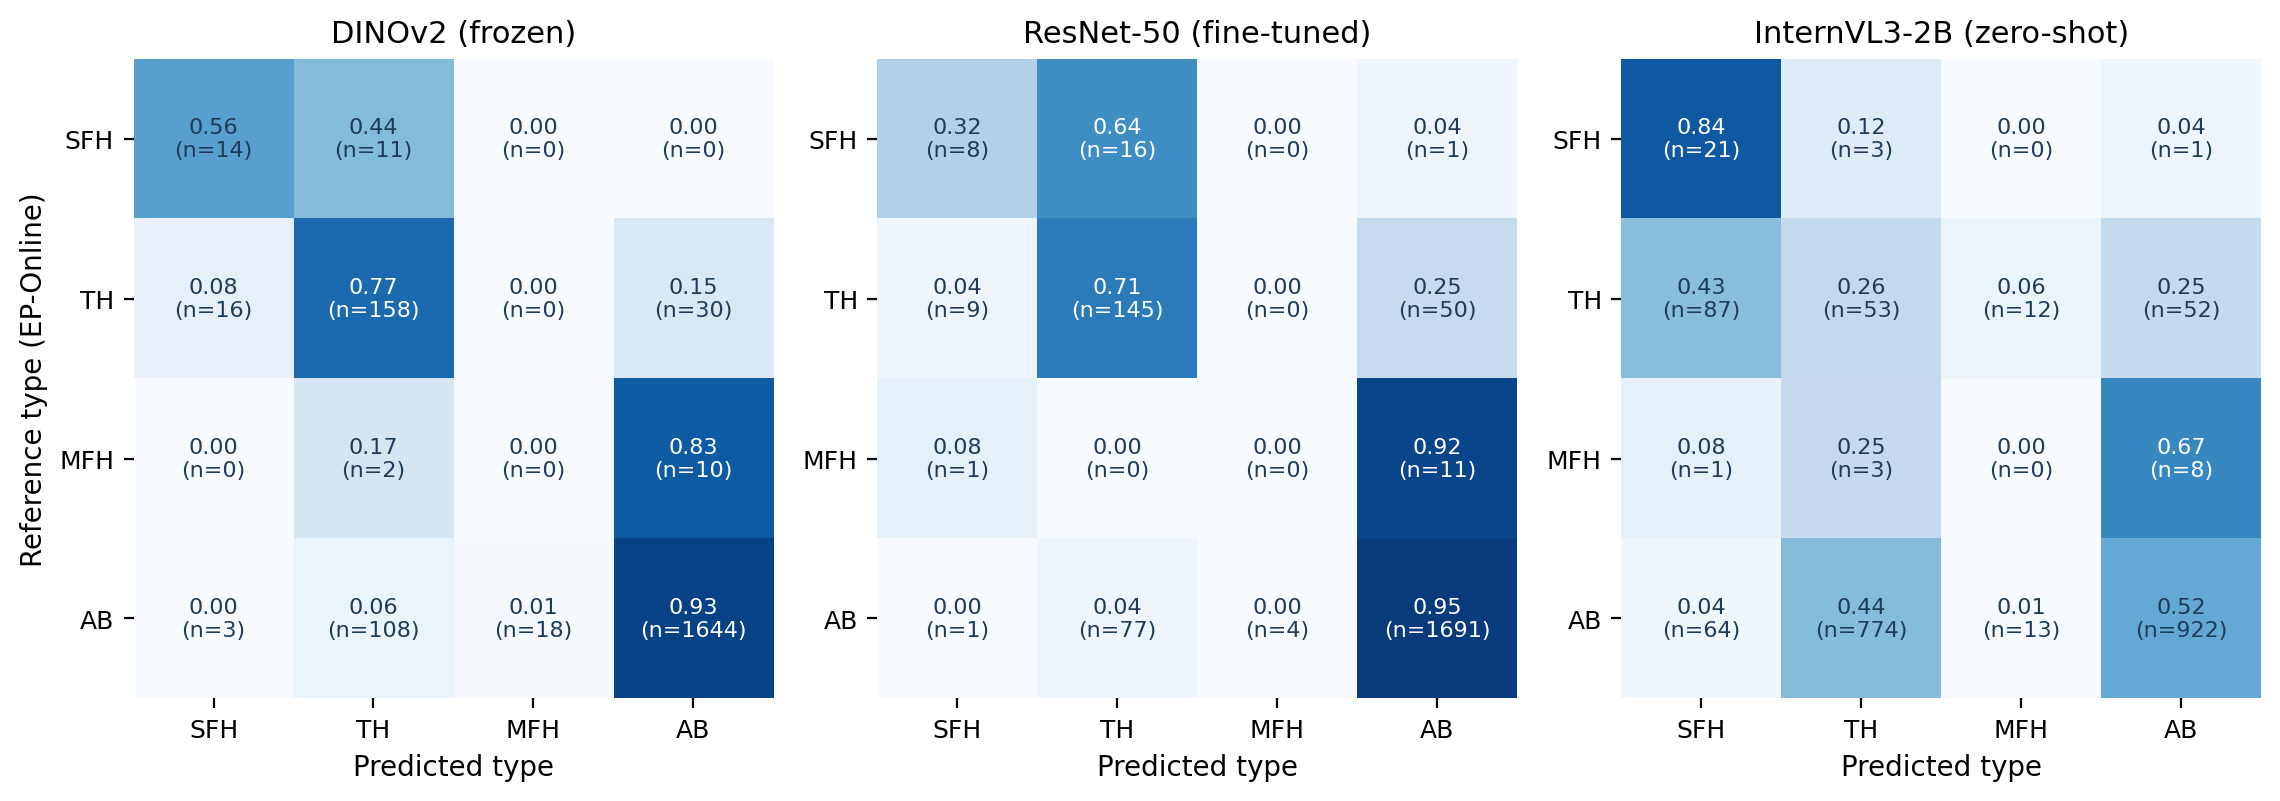
\includegraphics[width=\linewidth]{figures/fig/fig_4_2_type_confusion}
	\caption[Building type confusion matrices for the three vision configurations.]{Row-normalised building type confusion matrices for the three vision configurations on the evaluation set. Each cell also reports the number of buildings.}
	\label{fig:type_confusion}
\end{figure}

\paragraph{E1b: Construction year and \acs{TABULA} period.}
DINOv2 attained a year MAE of 9.40 years and an $R^2$ of 0.681, compared with 11.75 years and 0.551 for ResNet-50. InternVL3-2B had a year MAE of 30.65 years and a negative $R^2$. After mapping years to the six TABULA-NL periods, the corresponding period accuracies were 0.902, 0.893, and 0.769. Figure~\ref{fig:year_floor_scatter} shows that the largest deviations for the trained configurations occurred among newer buildings, whose predicted years were often earlier than their reference years.

\paragraph{E1c: Floor count.}
Floor count MAE was 0.375 for DINOv2, 0.425 for ResNet-50, and 0.708 for InternVL3-2B. Their $R^2$ values were 0.558, 0.542, and 0.010, respectively. The reference floor counts were concentrated between two and six, as shown in Figure~\ref{fig:year_floor_scatter}.

\begin{figure}[htbp]
	\centering
	\includegraphics[width=\linewidth]{figures/fig/fig_4_4_pred_vs_true_r2}
	\caption[Predicted and reference construction year and floor count.]{Predicted and reference construction year and floor count. Columns show DINOv2, ResNet-50, and InternVL3-2B; each panel reports MAE and $R^2$ on the evaluation set.}
	\label{fig:year_floor_scatter}
\end{figure}

Figure~\ref{fig:attribute_examples} presents six examples from the evaluation set to illustrate how the three vision configurations performed under different viewing conditions.
DINOv2 and ResNet-50 correctly predicted building type in the examples with partial occlusion and a distorted view. In contrast, all three configurations predicted an incorrect construction period for the examples with low image quality, a distorted view, and full occlusion. InternVL3-2B misclassified building type in one example with a clear view. Together, these cases show that correct predictions for one output did not ensure correct predictions for the others under the same viewing condition.

\begin{figure}[p]
	\centering
	\includegraphics[width=\linewidth]{../Thesis_reports/fig_ch4_svi_examples.png}
	\caption[Examples of attribute predictions under different image conditions.]{Selected examples from the evaluation set showing reference attributes and predictions from DINOv2, ResNet-50, and InternVL3-2B. Check marks indicate agreement in building type and \acs{TABULA} construction period. The examples illustrate clear views, occlusion, low image quality, and oblique viewpoints.}
	\label{fig:attribute_examples}
\end{figure}

\subsection{Experiment II Results: Archetype Assignment and Thermal Consequences}
\label{sec:joint_cell_assignment}

\paragraph{E2a: Joint archetype cell assignment.}
Table~\ref{tab:joint_cell} reports the joint cell results. DINOv2 and ResNet-50 reached joint accuracies of 0.826 and 0.827. The uniform expectation was 0.042, but the majority cell baseline was 0.791 because 1,594 of the 2,014 evaluated buildings occupied AB\,\textbar\,NL.01. Both trained configurations therefore exceeded the majority cell baseline by 0.035. InternVL3-2B reached 0.342.

\begin{table}[htbp]
	\centering
	\caption{Joint TABULA-NL cell assignment on the evaluation set.}
	\label{tab:joint_cell}
	\small
	\begin{tblr}{
		width = \linewidth,
		colspec = {X[l] Q[r,m,3.0cm] Q[r,m,3.4cm]},
		colsep = 4pt,
		row{1} = {font=\bfseries},
		rowsep = 2pt,
	}
		\toprule
		Vision configuration & Joint accuracy & Macro cell recall \\
		\midrule
		DINOv2, frozen backbone & 0.826 & \textbf{0.189} \\
		ResNet-50, full fine tuning & \textbf{0.827} & 0.135 \\
		InternVL3-2B, no parameter update & 0.342 & 0.168 \\
		\bottomrule
	\end{tblr}
	\par\vspace{0.4em}
	\begin{minipage}{\linewidth}
		\footnotesize\textit{Note.} All metrics are computed on the 2,014-building evaluation set. Expected uniform accuracy is 0.042. Majority cell accuracy is 0.791.
	\end{minipage}
\end{table}

Macro cell recall was 0.189 for DINOv2, 0.135 for ResNet-50, and 0.168 for InternVL3-2B. Figure~\ref{fig:cell_recall} shows that DINOv2 recalled 0.932 of AB\,\textbar\,NL.01 and 0.789 of TH\,\textbar\,NL.01, while recall for most cells after 1964 did not exceed 0.25. All MFH cells had zero recall. InternVL3-2B recovered some cells with one or two observations, which increased its macro cell recall despite its lower joint accuracy.

\begin{figure}[htbp]
	\centering
	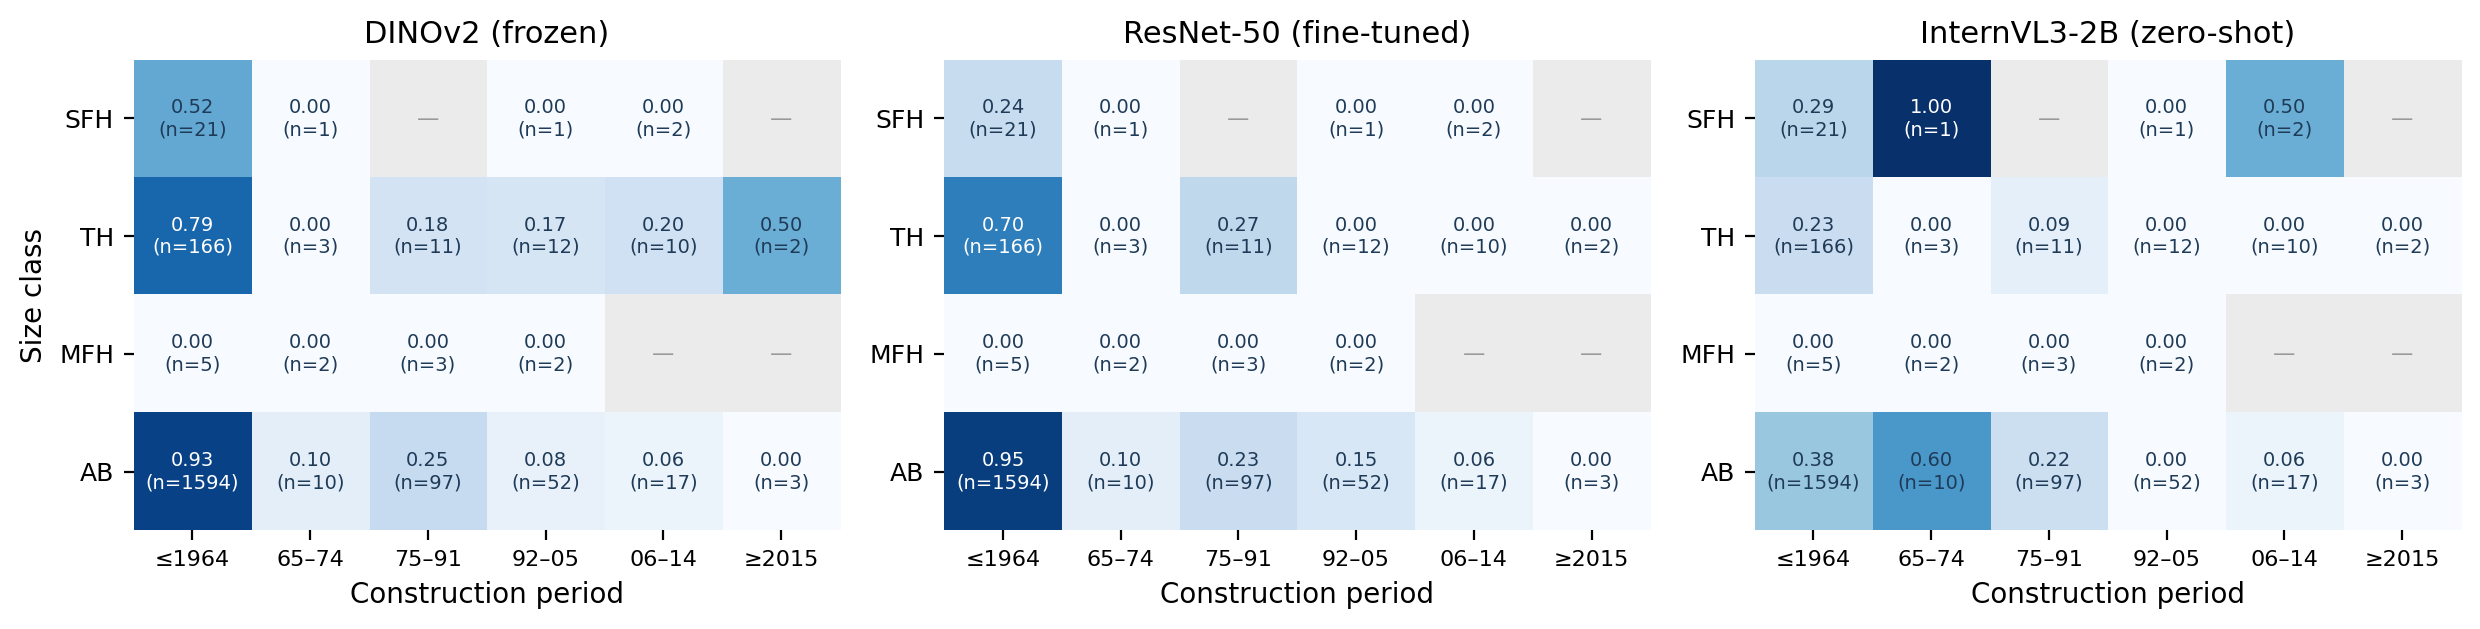
\includegraphics[width=\linewidth]{figures/fig/fig_4_3_cell_recall_heatmap}
	\caption[Recall across occupied TABULA-NL cells.]{Recall across occupied TABULA-NL cells in the evaluation set. Each cell reports recall and the number of reference buildings; cells without observations are grey.}
	\label{fig:cell_recall}
\end{figure}

\paragraph{E2b: Thermal consequences of cell assignment.}
Table~\ref{tab:htr_metrics} reports the difference between $h_{tr}$ values calculated from predicted and reference cells at $\mathrm{WWR}=0.25$. DINOv2 had an MAE of 0.149\,$\mathrm{W/(K\,m^2)}$ and an $R^2$ of 0.810. The corresponding values were 0.155 and 0.775 for ResNet-50, and 0.474 and 0.439 for InternVL3-2B. The separation in MAE between DINOv2 and InternVL3-2B was a factor of 3.2.

\begin{table}[htbp]
	\centering
	\caption{Thermal consequences of predicted archetype cells at $\mathrm{WWR}=0.25$.}
	\label{tab:htr_metrics}
	\footnotesize
	\begin{tblr}{
		width = \linewidth,
		colspec = {X[l] Q[r,m,3.0cm] Q[r,m,2.0cm] Q[r,m,3.0cm]},
		colsep = 3pt,
		row{1} = {font=\bfseries},
		rowsep = 2pt,
	}
		\toprule
		Vision configuration & $h_{tr}$ MAE ($\mathrm{W/(K\,m^2)}$) & $h_{tr}$ $R^2$ & Floor-area-weighted relative difference \\
		\midrule
		DINOv2, frozen backbone & \textbf{0.149} & \textbf{0.810} & $+9.8$\% \\
		ResNet-50, full fine tuning & 0.155 & 0.775 & $+10.2$\% \\
		InternVL3-2B, no parameter update & 0.474 & 0.439 & $+16.6$\% \\
		\bottomrule
	\end{tblr}
	\par\vspace{0.4em}
	\begin{minipage}{\linewidth}
		\footnotesize\textit{Note.} All metrics are computed on the 2,014-building evaluation set.
	\end{minipage}
\end{table}

All three configurations produced a positive floor-area-weighted relative difference from the reference cell calculations. The values ranged from $+9.8$\% for DINOv2 to $+16.6$\% for InternVL3-2B. Repeating the calculation at WWR values of 0.15, 0.25, and 0.35 left the ranking unchanged. The DINOv2 and ResNet-50 MAEs were 0.149 and 0.155 at all three WWR values at the reported precision, while the InternVL3-2B MAE changed from 0.495 to 0.453. Table~\ref{tab:wwr_sensitivity} reports the complete sensitivity results.

Experiment II therefore shows that similar overall joint accuracy for the two trained configurations corresponded to similar thermal differences, while the lower InternVL3-2B joint accuracy coincided with a substantially larger $h_{tr}$ difference.

\subsection{Experiment III Results: Energy Class Prediction}
\label{sec:energy_class_condition_comparison}

Experiment III compares all energy class prediction conditions on the 2,014-building evaluation set. Results for the primary binary target are presented first, followed by the seven-class target and feature contribution analysis.

\paragraph{E3a: Binary energy class prediction.}
Table~\ref{tab:binary_conditions} reports the default threshold results. Direct image prediction with DINOv2 attained the highest macro F1 at 0.597 and the highest macro recall at 0.601. Direct image prediction with ResNet-50 followed with a macro F1 of 0.566. The reference attribute condition reached 0.492, while predicted attributes from DINOv2 and ResNet-50 reached 0.490 and 0.488.

\begin{table}[htbp]
	\centering
	\caption{Binary energy class prediction on the evaluation set ($n=2{,}014$).}
	\label{tab:binary_conditions}
	\footnotesize
	\begin{tblr}{
		width = \linewidth,
		colspec = {Q[l,m,3.0cm] X[l] Q[r,m,1.9cm] Q[r,m,1.7cm] Q[r,m,1.5cm]},
		colsep = 3pt,
		row{1} = {font=\bfseries},
		rowsep = 2pt,
	}
		\toprule
		Condition & Vision configuration & Macro precision & Macro recall & Macro F1 \\
		\midrule
		Uniform random & Analytic expectation & 0.500 & 0.500 & 0.479 \\
		Reference attributes & LightGBM & \textbf{0.612} & 0.529 & 0.492 \\
		Direct image & DINOv2 & 0.595 & \textbf{0.601} & \textbf{0.597} \\
		Direct image & ResNet-50 & 0.566 & 0.566 & 0.566 \\
		Direct image & InternVL3-2B & 0.149 & 0.500 & 0.230 \\
		Predicted attributes & DINOv2 & 0.566 & 0.522 & 0.490 \\
		Predicted attributes & ResNet-50 & 0.550 & 0.518 & 0.488 \\
		Predicted attributes & InternVL3-2B & 0.527 & 0.528 & 0.527 \\
		\bottomrule
	\end{tblr}
\end{table}

The reference attribute condition recalled 96.0\% of classes A to C but 9.8\% of classes D to G. Predicted attributes from DINOv2 and ResNet-50 produced similar recalls of 10.8\% and 11.0\% for classes D to G. Direct DINOv2 increased recall for this group to 46.9\%. Direct InternVL3-2B assigned every building to classes D to G, so its macro F1 of 0.230 reflected a constant prediction rather than discrimination among buildings. Table~\ref{tab:binary_perclass} reports precision, recall, and F1 for both class groups.

\paragraph{E3b: Seven-class energy prediction.}
Table~\ref{tab:sevenclass_conditions} reports results for classes A to G. Direct DINOv2 attained the highest macro F1 at 0.213, followed by direct ResNet-50 at 0.201. The reference attribute condition reached 0.171 and the three predicted attribute conditions ranged from 0.131 to 0.151. The metric ranking differed for exact and $\pm1$ accuracy, for which the reference attribute condition attained the highest values of 0.358 and 0.660.

\begin{table}[htbp]
	\centering
	\caption{Seven-class energy class prediction on the evaluation set ($n=2{,}014$).}
	\label{tab:sevenclass_conditions}
	\small
	\begin{tblr}{
		width = \linewidth,
		colspec = {X[l] X[l] Q[r,m,2.1cm] Q[r,m,2.1cm] Q[r,m,2.1cm]},
		colsep = 4pt,
		row{1} = {font=\bfseries},
		rowsep = 2pt,
	}
		\toprule
		Condition & Vision configuration & Macro F1 & Exact accuracy & $\pm1$ accuracy \\
		\midrule
		Uniform random & Analytic expectation & 0.127 & 0.143 & 0.390 \\
		Reference attributes & LightGBM & 0.171 & \textbf{0.358} & \textbf{0.660} \\
		Direct image & DINOv2 & \textbf{0.213} & 0.266 & 0.544 \\
		Direct image & ResNet-50 & 0.201 & 0.263 & 0.570 \\
		Direct image & InternVL3-2B & 0.015 & 0.046 & 0.167 \\
		Predicted attributes & DINOv2 & 0.151 & 0.297 & 0.589 \\
		Predicted attributes & ResNet-50 & 0.148 & 0.284 & 0.588 \\
		Predicted attributes & InternVL3-2B & 0.131 & 0.277 & 0.596 \\
		\bottomrule
	\end{tblr}
\end{table}

Only the reference attribute condition exceeded the majority baseline of 0.612 for $\pm1$ accuracy. Direct InternVL3-2B predicted class F for approximately 99\% of the evaluation set and consequently remained below the uniform expectation for all three seven-class metrics. These results close the main comparison by showing that condition ranking depends on both target resolution and evaluation metric.

\paragraph{E3c: Feature contribution analysis.}
The leave-one-out results in Table~\ref{tab:feature_ablation} identify construction year as the largest contributor among the eight inputs of the reference attribute classifier. Removing year reduced macro F1 by 0.032 for the seven-class target and 0.030 for the binary target. Removing the four TABULA U-values changed macro F1 by less than 0.003 in either target. Adding all four clean reconstructed geometry features increased macro F1 by 0.039 for the seven-class target and 0.104 for the binary target.

\begin{table}[htbp]
	\centering
	\caption{Changes in development set macro F1 under feature removal and clean geometry augmentation.}
	\label{tab:feature_ablation}
	\small
	\begin{tblr}{
		width = \linewidth,
		colspec = {X[l] Q[r,m,3.7cm] Q[r,m,3.2cm]},
		colsep = 4pt,
		row{1} = {font=\bfseries},
		rowsep = 2pt,
	}
		\toprule
		Feature change & Seven-class $\Delta$ macro F1 & Binary $\Delta$ macro F1 \\
		\midrule
		Remove construction year & $\mathbf{-0.032}$ & $\mathbf{-0.030}$ \\
		Remove floor count & $-0.012$ & $-0.011$ \\
		Remove building type & $-0.003$ & $+0.003$ \\
		Remove four TABULA U-values & $-0.000$ & $+0.002$ \\
		Remove study area & $-0.009$ & $-0.006$ \\
		Add reconstructed shape factor & $+0.025$ & $+0.063$ \\
		Add reconstructed floor area & $+0.025$ & $+0.071$ \\
		Add all four clean 3DBAG geometry features & $+0.039$ & $+0.104$ \\
		\bottomrule
	\end{tblr}
	\par\vspace{0.4em}
	\begin{minipage}{\linewidth}
		\footnotesize\textit{Note.} The full feature baselines were 0.181 for the seven-class target and 0.478 for the binary target. Geometry additions use only reconstructed 3DBAG fields; certificate geometry fields identified by the provenance audit are excluded.
	\end{minipage}
\end{table}

Experiment III therefore yields three principal findings. Direct DINOv2 produced the highest macro F1 for both energy class targets. Replacing reference attributes with predicted building attributes changed binary macro F1 by less than 0.005 but reduced seven-class macro F1 by approximately 0.019. The feature analysis identifies construction year as the strongest contributor among the structured inputs and shows that clean reconstructed geometry adds information not captured by the main input set.

\section{Discussion}
\label{sec:discussion}

The discussion follows the correspondence between the method stages, experiments, and Results subsections established in Table~\ref{tab:experiment_correspondence}. Experiment I interprets the accuracy and failure patterns of building attribute prediction from \Ac{SVI}. The effects of prediction errors on TABULA-NL archetype assignment and thermal parameters are examined through Experiment II. Experiment III compares registered energy class prediction across the reference attribute, predicted attribute, and direct image conditions and examines the contribution of the structured inputs.

\subsection{Building Attribute Prediction}

DINOv2 used a pretrained self-supervised backbone whose parameters remained fixed, while the MLP and three attribute heads were trained on the development data. For building type prediction, DINOv2 and ResNet-50 achieved similar accuracies of 0.902 and 0.916, respectively. However, DINOv2 achieved a slightly higher macro F1 of 0.522 than the 0.495 achieved by ResNet-50, showing better performance for the less frequent SFH and TH classes. Because only the MLP and attribute heads were updated, DINOv2 had fewer trainable parameters than the fully fine-tuned ResNet-50. This combination of stronger performance for the less frequent classes and fewer trainable parameters supports using the DINOv2 configuration to enrich missing building attributes from \Ac{SVI} when labelled development data are limited.

Construction year was the strongest continuous prediction target for DINOv2, with an $R^2$ of 0.681. This value is close to the 0.710 reported by \textcite{liang2025} for a fully fine-tuned InternVL3-2B model, but the datasets, label sources, and training procedures differ, so the values are not a direct benchmark. The negative $R^2$ of the InternVL3-2B configuration in this study instead shows that prompting without parameter updates did not recover building-level year variation among the evaluated Dutch buildings. The selected examples further suggest that visibility, occlusion, and viewpoint are relevant failure conditions, although a systematic image quality experiment would be required to quantify their effects.

\subsection{Archetype Assignment and Thermal Consequences}

The joint cell result requires interpretation against both baselines. Joint accuracies above 0.82 appear high relative to uniform assignment, but the majority cell alone reaches 0.791 because the evaluation set is dominated by old apartment blocks. Macro cell recall remained below 0.19 for both trained configurations, showing that their high joint accuracy did not extend evenly to less frequent combinations of building type and construction period. Earlier energy modelling studies identified building type and construction period as sources of error \parencite{dochev2020,bass2022}. Experiment II extends this evidence by quantifying how errors in attributes predicted from images change TABULA-NL cell assignment for the same buildings.

The $h_{tr}$ comparison distinguishes cell errors by their thermal consequence. It separated DINOv2 from InternVL3-2B more clearly than joint accuracy. All three predicted cell sets produced higher aggregate transmission heat transfer coefficients than the reference assignments. The construction year scatter provides a plausible explanation. Several newer buildings were assigned to earlier periods with higher representative U-values, increasing the calculated $h_{tr}$.

\subsection{Energy Class Prediction}

For the binary target, the direct image and predicted attribute conditions based on DINOv2 and ResNet-50 exceeded the uniform random expectation for all three reported metrics. Replacing reference attributes with attributes predicted by DINOv2 reduced macro precision by 0.046, from 0.612 to 0.566, while macro F1 changed by only 0.002, from 0.492 to 0.490. The ResNet-50 predicted attribute condition produced a similar macro F1 of 0.488. These small differences indicate that attributes predicted from \Ac{SVI} retained most of the binary prediction performance available from reference attributes. However, the reference and trained predicted attribute conditions recalled only around 10\% of classes D to G. 

Direct DINOv2 achieved a macro F1 of 0.597, exceeding the 0.492 obtained by the reference attribute condition. Earlier studies similarly found that \Ac{SVI} contains information associated with registered energy performance \parencite{mayer2023uk,mayer2023dk}. The higher macro F1 therefore indicates that the complete direct DINOv2 procedure captured visual cues associated with registered energy class. 

 InternVL3-2B produced the weakest building attribute results and performed poorly when applied directly to both energy class targets. These results indicate that prompt design without parameter updating did not extract reliable energy class information from the evaluated \Ac{SVI}. Further training with local images and registered energy class labels may therefore be required.

The seven-class target reveals a clearer limitation. Macro F1 remained low for every condition, indicating that none of the evaluated procedures reliably distinguished all seven registered classes. The DINOv2 predicted attribute condition reached a $\pm1$ accuracy of 0.589, which was 0.071 below the reference attribute condition. However, its $\pm1$ accuracy remained below the majority baseline of 0.612. The results therefore suggest that predictions often remained near the registered class, but adjacent energy classes could not be separated reliably.

The feature analysis helps explain the limited performance of the structured conditions. Construction year provided the largest contribution among the eight inputs, while the deterministic TABULA-NL U-values added little information once building type and construction period were included. Reconstructed geometry improved macro F1 for both targets, showing that the main structured input set omitted relevant building information. Overall, Experiment III shows that \Ac{SVI} can preserve much of the binary prediction performance through predicted attributes. 

\subsection{Validity, Limitations, and Future Evaluation}
\label{sec:validity_limitations}

The evaluated buildings limits geographic transfer. Mapillary coverage and image filtering produced a dataset dominated by Amsterdam and AB buildings, with few examples in several building types, construction periods, archetype cells, and registered energy classes. Performance may therefore reflect this distribution. Future geographic evaluation should exclude each study area from model development in turn and report the composition and class-specific performance of every target set. 

Target validity is constrained by the difference between the certificate and analysis units. EP-Online certificates refer to dwellings, whereas the analysis uses BAG buildings. Multiple certificates were linked to 58.4\% of the 10,086 buildings, and 77.1\% of this group had inconsistent registered energy classes. Selecting the most recent certificate provides one reproducible target but may represent only one dwelling or registration date. Future evaluation should compare latest and modal class targets and align certificate and image dates.

Model performance may be improved further because hyperparameters were not exhaustively optimised for each prediction target, and InternVL3-2B was evaluated without parameter updating. Future experiments should include an open-source \ac{VLM} fine-tuned on the experimental data, class imbalance treatments, calibration analysis, and systematic hyperparameter optimisation.

The archetype and thermal results describe assigned properties and their calculated thermal implications, while measured building performance lies outside the scope of this analysis. \Ac{SVI} may show visible facade or window changes but cannot verify concealed insulation, heating system upgrades, or renovations within individual units. The thermal comparison also relies on reconstructed 3DBAG geometry, a fixed WWR range, and archetype U-values rather than measured envelope properties. Future physical evaluation should incorporate verified renovation records, measured envelope properties, and independent heat demand observations. 

Overall, \Ac{SVI} can provide useful building attributes when reference building attributes are missing, and those attributes can be connected to a transparent archetype workflow. For the evaluated energy class task, however, building type, construction year, floor count, and their TABULA-NL U-values do not contain all information required for class-balanced prediction. A practical workflow should use administrative records and reconstructed geometry where they are available, use \ac{SVI} to supplement building attributes that can be inferred from visible facades.

\chapter{Conclusions}
\label{ch:conclusions}

This thesis examined whether \ac{SVI} can provide building attributes that are useful for building energy assessment when administrative records are incomplete.
The question was investigated through a Dutch case in which building type, construction year, and floor count predicted from \ac{SVI} were compared with reference building attributes, used for TABULA-NL archetype assignment, and evaluated as inputs to registered energy class prediction.
TABULA-NL therefore provides the archetype framework used to assess the usefulness and consequences of image-based attribute enrichment rather than the overarching goal of the thesis.

\section{Conclusions}
\label{sec:conclusions}

Objective~1 assessed the predictive performance of \ac{SVI} for building type, construction year, and floor count.
The three vision configurations produced predictions for all three attributes, but prediction quality differed by attribute, class, and vision configuration.
DINOv2 with a frozen backbone produced the most consistent overall results, achieving the best value in six of the seven principal attribute metrics.
ResNet-50 attained the highest building type accuracy, but this result was influenced by strong performance for the dominant Apartment Block class, while DINOv2 achieved higher macro F1 and stronger recall for less frequent classes.
InternVL3-2B without parameter updating did not provide sufficient accuracy for the three attribute tasks in the evaluated setup.

Objective~2 quantified how errors in predicted building type and construction year affect TABULA-NL archetype assignment and the associated thermal parameters.
DINOv2 and ResNet-50 achieved joint cell accuracies of 0.826 and 0.827, respectively, but the majority cell baseline already reached 0.791.
Their macro cell recalls of 0.189 and 0.135 show that the high overall agreement was concentrated in frequent combinations of building type and construction period rather than distributed across the occupied archetype cells.
The errors also changed the assigned thermal parameters.
Relative to calculations based on reference cells, the cells assigned from DINOv2 and ResNet-50 predictions produced aggregate transmission heat transfer coefficients that were 9.8\% and 10.2\% higher, while InternVL3-2B produced a value 16.6\% higher.
These comparisons quantify the effect of attribute errors on archetype assignment, but they do not validate the assigned parameters against measured envelope properties or heat demand.

Objective~3 determined how the source of building information affects registered energy class prediction.
Changing from reference attributes to DINOv2 predicted attributes reduced binary macro F1 by only 0.002, but reduced seven-class macro F1 by 0.019.
The small binary difference does not indicate reliable classification because both attribute conditions had low recall for classes D to G.
Direct image prediction with DINOv2 achieved the highest macro F1 for both targets, reaching 0.597 for the binary task and 0.213 for the seven-class task.
This result indicates that the images contain information relevant to the registered energy class that is not represented by building type, construction year, floor count, and the corresponding TABULA-NL U-values alone.
Among the structured inputs, construction year made the largest marginal contribution to energy class prediction and should therefore be prioritised when improving building attribute prediction from \ac{SVI}.

Overall, the findings support \ac{SVI} as a supplementary source of building information rather than a universal replacement for administrative records.
When reference building attributes are incomplete, predictions of building type, construction year, and floor count can support preliminary building stock assessment and targeted data collection because the predicted attributes can be inspected before archetype assignment and used in subsequent analyses.
Administrative records and reconstructed geometry should remain the preferred sources where they are available, while \ac{SVI} can supplement building attributes that can be inferred from visible facades.
When the registered energy class is the only required output, direct image prediction provided stronger class-balanced performance than prediction based on the evaluated structured inputs.
However, neither procedure should replace an \ac{EPC}, a physical survey, or measured performance assessment.
The appropriate use of \ac{SVI} therefore depends on whether the application requires building attributes, archetype parameters, or an energy class prediction.

\section{Contributions}
\label{sec:contributions}

This thesis makes three contributions to the evaluation of building attributes predicted from \ac{SVI} for building stock enrichment.
These contributions concern the controlled assessment of attribute sources and their consequences for archetype assignment and energy class prediction rather than the development of a new predictive architecture.

\textbf{The first contribution is a controlled evaluation of building attribute prediction from SVI.}
The comparison evaluates a fully fine-tuned ResNet-50, a frozen DINOv2 backbone with supervised prediction layers, and InternVL3-2B without parameter updating using one predefined holdout set and the same attribute definitions.
The two supervised configurations produced predictions for all 2,018 holdout buildings, while two invalid InternVL3-2B records were excluded from its metrics. This design identifies the strengths and limitations of each complete configuration without implying that every metric has the same denominator.

\textbf{The second contribution connects attribute errors to archetype assignment and thermal parameters.}
The building-level dataset links Mapillary imagery, reference building attributes, reconstructed 3DBAG geometry, \ac{EPC} records, and TABULA-NL archetypes and identifies the data source of each field.
Predicted building type and construction year are used to assign the joint archetype cell and its U-values, which are then included in the calculation of the floor-area-normalised transmission heat transfer coefficient $h_{tr}$.
This structure separates attribute prediction errors from their effects on cell agreement, assigned thermal parameters, and aggregate transmission heat transfer.

\textbf{The third contribution is a controlled comparison of information sources for energy class prediction.}
Reference and predicted building attributes are compared on the 2,014-building evaluation set using the same fitted classifier.
Direct image prediction is evaluated as a separate procedure that does not produce intermediate building attributes.
The comparison therefore shows how energy class results change with the source and representation of building information, while feature ablation identifies the contribution of the structured inputs.


%============ Anhang =============================================================
\begin{appendix}
\chapter{Data Definitions and Source Provenance}
\label{ch:appendix_a}

This appendix defines the 3DBAG variables, evaluation-set exclusions, and TABULA-NL source decisions needed to reproduce the dataset construction, evaluation, and archetype lookup.
Section~\ref{sec:appendix_a_3dbag} distinguishes the floor count used as a reference attribute from the geometric variables derived for physical calculations and feature analysis.
Section~\ref{sec:appendix_a_evaluation_set} documents the records excluded when the fixed holdout set is reduced to the evaluation set.
Section~\ref{sec:appendix_a_tabula} documents how the operational TABULA-NL lookup was generated and how a difference between the source workbook and the WebTool was resolved.

\section{3DBAG Variables}
\label{sec:appendix_a_3dbag}

3DBAG provides automatically reconstructed geometry rather than surveyed measurements \parencite{threedbagdocs,peters2022,dukai2021}.
Table~\ref{tab:3dbag_fields} separates the reference floor count used in attribute prediction from the geometric variables derived from reconstructed surfaces and heights.
This distinction is necessary because the reference floor count and the floor count used to derive total floor area use different height fields when \texttt{b3\_bouwlagen} is unavailable.

\begin{table}[htbp]
	\centering
	\caption{Definitions and analytical roles of the 3DBAG variables used in this study.}
	\label{tab:3dbag_fields}
	\footnotesize
	\begin{tblr}{
			width = \linewidth,
			colspec = {Q[l,m,3.3cm] X[l] X[l]},
			colsep = 4pt,
			row{1} = {font=\bfseries},
			rowsep = 2pt,
		}
		\toprule
		Variable & Definition & Role in the analysis \\
		\midrule
		Reference floor count & \texttt{b3\_bouwlagen}; if missing, \texttt{round(b3\_h\_50p / 3.0)} & Reference target for floor count prediction \\
		Volume & \texttt{b3\_volume\_lod22} & Reconstructed building volume used in the geometry feature analysis \\
		Envelope area & Sum of exterior wall, flat roof, sloped roof, and ground surface areas; party walls are excluded & Exterior envelope area used to calculate shape factor \\
		Building height & Maximum of zero and \texttt{b3\_h\_max} $-$ \texttt{b3\_h\_maaiveld} & Reconstructed height used when deriving geometric floor count \\
		Geometric floor count & \texttt{b3\_bouwlagen}; if missing, the maximum of one and \texttt{round(building\_height / 3.0)} & Intermediate variable used to derive total floor area \\
		Estimated floor area & \texttt{b3\_opp\_grond} $\times$ \texttt{num\_floors\_estimated} & Floor area used to normalise transmission heat transfer and in the geometry feature analysis \\
		Shape factor & \texttt{envelope\_area / volume} & Exterior surface to volume ratio used in the geometry feature analysis \\
		Shared wall ratio & Party wall area divided by the sum of exterior and party wall areas & Measure of attached wall exposure used in the geometry feature analysis \\
		\bottomrule
	\end{tblr}
\end{table}

The transmission heat transfer calculation uses reconstructed element areas directly and uses \texttt{floor\_area\_estimated} as its denominator.
The geometry feature analysis uses volume, estimated floor area, shape factor, and shared wall ratio as additions to the structured energy class model.
None of these variables is interpreted as a field measurement of the current building envelope.

\section{Evaluation Set Eligibility}
\label{sec:appendix_a_evaluation_set}

The fixed holdout set contains 2,018 buildings, while the performance comparisons use an evaluation set of 2,014 buildings with complete outputs from all three vision configurations and reconstructed areas suitable for the thermal calculation. Reconstructed areas satisfy the validity criteria when estimated floor area is between 20 and 100,000\,m$^2$, exterior wall area is between 1 and 50,000\,m$^2$, and ground area is between 5 and 20,000\,m$^2$. Table~\ref{tab:evaluation_set_exclusions} documents the four excluded buildings. The two exclusion groups do not overlap.

\begin{table}[htbp]
	\centering
	\caption{Buildings excluded from the fixed holdout set when defining the evaluation set.}
	\label{tab:evaluation_set_exclusions}
	\small
	\begin{tblr}{
		width = \linewidth,
		colspec = {Q[l,m,3.8cm] Q[l,m,2.3cm] X[l]},
		colsep = 4pt,
		row{1} = {font=\bfseries},
		rowsep = 3pt,
	}
		\toprule
		\texttt{pand\_id} & Study area & Exclusion reason \\
		\midrule
		\texttt{0599100000240334} & Rotterdam & InternVL3-2B did not return complete predictions for building type, construction year, and floor count \\
		\texttt{0599100000647213} & Rotterdam & InternVL3-2B did not return complete predictions for building type, construction year, and floor count \\
		\texttt{0363100012160228} & Amsterdam & Reconstructed ground and estimated floor areas were below the validity ranges \\
		\texttt{0599100000700053} & Rotterdam & Estimated floor area exceeded the validity range \\
		\bottomrule
	\end{tblr}
\end{table}

\section{TABULA-NL Lookup Provenance}
\label{sec:appendix_a_tabula}

The operational TABULA-NL lookup was generated from the \texttt{Tab.Building.Constr} sheet of the TABULA values workbook and checked against the Dutch exemplary building records in the TABULA WebTool \parencite{loga2016,tabulawebtool}.
The generator selects existing state construction assemblies for each residential size class and construction period.
Terraced houses use the solid wall variants, while single family houses, multifamily houses, and apartment blocks use the cavity wall variants represented by the corresponding exemplary buildings.
When the workbook contains several subperiod assemblies within one TABULA-NL period, the implementation selects the assembly with the highest U-value. Window U-values are assigned directly by construction period.

This value is used consistently in Table~\ref{tab:tabula_uvalues} and in all archetype and transmission heat transfer calculations.
The generated lookup and its element source mapping are stored in \texttt{data/processed/tabula\_nl.csv} and \texttt{data/processed/tabula\_nl\_provenance.csv}.

\chapter{Model Training and Inference Settings}
\label{ch:appendix_b}

This appendix reports the settings needed to reproduce the attribute and energy class models.
Section~\ref{sec:appendix_b_vision_configs} describes the two trained attribute models, Section~\ref{sec:appendix_b_direct_energy} specifies the direct image energy class models, and Section~\ref{sec:appendix_b_lightgbm} reports the \acs{LightGBM} configuration used with structured inputs.
The sections distinguish settings shared across configurations from decisions that apply to one model only.
All model training and \ac{VLM} inference used one NVIDIA GeForce RTX 4060 Laptop graphics processing unit with 8\,GB of video memory.

\section{Attribute Prediction Models}
\label{sec:appendix_b_vision_configs}

The ResNet-50 and DINOv2 attribute models share the same prediction heads, image transformations, training duration, and checkpoint selection rule, but differ in the parameters updated and in optimiser grouping.
Both models use AdamW with a nominal weight decay of 0.01 and cosine annealing with \(T_{\max}=30\).
For ResNet-50, parameter grouping excludes biases and one-dimensional normalisation parameters from weight decay.
For DINOv2, weight decay is applied to all trainable parameters in the multilayer perceptron and output heads.
Training stops after a maximum of 30 epochs or after validation building type macro F1 fails to improve for 10 epochs.
Both models use fp16 automatic mixed precision.

Input images are resized to \(224 \times 224\) pixels and normalised using ImageNet statistics, with a mean of (0.485, 0.456, 0.406) and a standard deviation of (0.229, 0.224, 0.225).
Training augmentation comprises \texttt{RandomResizedCrop} with a scale range from 0.7 to 1.0, horizontal flipping with \(p=0.5\), and \texttt{ColorJitter} with brightness, contrast, and saturation set to 0.2.
Validation and holdout inference resize the short side to 256 pixels before applying a 224 pixel centre crop.
Building type cross entropy is weighted inversely to the frequencies of SFH, TH, MFH, and AB within each training fold.
Construction year and floor count are standardised using the mean and standard deviation of the training fold before mean squared error is calculated.

\begin{table}[htbp]
	\centering
	\caption{Training settings of the two attribute prediction models.}
	\label{tab:vision_hyperparams}
	\footnotesize
	\begin{tblr}{
			width = \linewidth,
			colspec = {Q[l,m,3.8cm] X[l] X[l]},
			colsep = 4pt,
			row{1} = {font=\bfseries},
			rowsep = 2pt,
		}
		\toprule
		Setting & ResNet-50 full fine tuning & Frozen DINOv2 \acs{ViT}-B/14 \\
		\midrule
		Pretrained weights (\texttt{timm}) & \texttt{resnet50} (ImageNet) & \texttt{vit\_base\_\allowbreak patch14\_\allowbreak dinov2.\allowbreak lvd142m} \\
		Backbone feature dimension & 2048 & 768 \\
		Attribute \acs{MLP} & Linear (2048 \(\rightarrow\) 256) + GELU + Dropout 0.3 & Linear (768 \(\rightarrow\) 256) + GELU + Dropout 0.3 \\
		Parameters updated & Backbone, attribute \acs{MLP}, and output heads & Attribute \acs{MLP} and output heads only \\
		Total parameters & 24.03\,M & 85.92\,M \\
		Trainable parameters & 24.03\,M (100\%) & 0.20\,M (approximately 0.2\%) \\
		Learning rate & Backbone \(1\times10^{-4}\); \acs{MLP} and heads \(5\times10^{-4}\) & \(5\times10^{-4}\) \\
		Batch size in buildings & 8 & 32 \\
		Optimiser and weight decay & AdamW; 0.01 with parameter grouping & AdamW; 0.01 on all trainable parameters \\
		Learning rate schedule & Cosine annealing (\(T_{\max}=30\)) & Cosine annealing (\(T_{\max}=30\)) \\
		Maximum epochs and patience & 30; 10 & 30; 10 \\
		Mixed precision & fp16 & fp16 \\
		Padding treatment & Only valid images enter the backbone & Zero padding with masked feature pooling \\
		\bottomrule
	\end{tblr}
\end{table}

Table~\ref{tab:vision_hyperparams} therefore reports the settings that differ between the two attribute models, while the preceding text defines their shared image processing and training rules.

\section{Direct Image Energy Class Models}
\label{sec:appendix_b_direct_energy}

The direct ResNet-50 classifier uses the ResNet-50 optimisation and image processing settings reported in Table~\ref{tab:vision_hyperparams}.
Its three attribute heads are replaced by one energy class classification head, and validation energy class macro F1 determines checkpoint selection.
Class weighted cross entropy is calculated from the energy class frequencies in each training fold.

The direct DINOv2 classifier uses the pretrained DINOv2 ViT-B/14 backbone but first caches one mean feature vector for each building.
A separate network with a 768 dimensional input, a 256 dimensional hidden layer, GELU activation, Dropout 0.3, and one energy class output head is trained on the cached features.
Training uses class weighted cross entropy, AdamW, a learning rate of \(5\times10^{-4}\), weight decay of 0.01, cosine annealing, a minibatch size of 256, and early stopping with a patience of 10 epochs.
Because the image features are computed before classifier training, image augmentation is not applied during this stage.

InternVL3-2B predicts the energy class from each of the three selected images without parameter updates.
Its output is aggregated at building level according to the rules in Appendix~\ref{ch:appendix_d}.
These descriptions define three complete direct image configurations rather than attributing their differences to one isolated model component.

\section{LightGBM Energy Class Models}
\label{sec:appendix_b_lightgbm}

Table~\ref{tab:lightgbm_hyperparams} reports the fixed \acs{LightGBM} configuration used with structured inputs.
The same settings are applied to all attribute input conditions, which limits their comparison to changes in the supplied building information.

\begin{table}[htbp]
	\centering
	\caption{Fixed LightGBM settings used for both energy class tasks and all attribute input conditions.}
	\label{tab:lightgbm_hyperparams}
	\small
	\begin{tblr}{
			width = \linewidth,
			colspec = {Q[l,m,5.0cm] X[l]},
			colsep = 4pt,
			row{1} = {font=\bfseries},
			rowsep = 2pt,
		}
		\toprule
		Hyperparameter & Value \\
		\midrule
		\texttt{objective} & \texttt{multiclass} for seven classes or \texttt{binary} for two class groups \\
		\texttt{n\_estimators} & 400 \\
		\texttt{learning\_rate} & 0.05 \\
		\texttt{num\_leaves} & 31 \\
		\texttt{max\_depth} & \(-1\), without a fixed maximum depth \\
		\texttt{min\_child\_samples} & 20 \\
		\texttt{subsample} & 0.8 \\
		\texttt{subsample\_freq} & 1 \\
		\texttt{colsample\_bytree} & 0.8 \\
		\texttt{reg\_lambda} & 1.0 \\
		\texttt{class\_weight} & None \\
		\texttt{random\_state} & 42 \\
		\bottomrule
	\end{tblr}
\end{table}

Only the objective changes between the binary and seven-class tasks.
No separate hyperparameter search is performed for individual input conditions.

\chapter{Supplementary Evaluation Results}
\label{ch:appendix_c}

This appendix reports two supporting analyses referenced in Chapter~\ref{ch:experiments}.
Section~\ref{sec:appendix_c_wwr} examines whether the assumed window-to-wall ratio changes the comparison of archetype assignments.
Section~\ref{sec:appendix_c_binary} reports class-level precision, recall, and F1 for the binary energy class task.
These tables provide the detailed evidence for patterns summarised in the main results.

\section{Window-to-Wall Ratio Sensitivity}
\label{sec:appendix_c_wwr}

Table~\ref{tab:wwr_sensitivity} reports the transmission heat transfer MAE after repeating the calculation with window-to-wall ratios of 0.15, 0.25, and 0.35.
The same reference and predicted archetype assignments are used at each ratio, allowing the calculation to isolate sensitivity to the assumed division between opaque wall and window area.

\begin{table}[htbp]
	\centering
	\caption[Sensitivity of the \(h_{tr}\) MAE to the assumed window-to-wall ratio.]{Sensitivity of the \(h_{tr}\) MAE (\(\mathrm{W/(K\,m^2)}\)) to the assumed window-to-wall ratio.}
	\label{tab:wwr_sensitivity}
	\small
	\begin{tblr}{
			width = \linewidth,
			colspec = {X[l] Q[r,m,2.4cm] Q[r,m,2.4cm] Q[r,m,2.4cm]},
			colsep = 4pt,
			row{1} = {font=\bfseries},
			rowsep = 2pt,
		}
		\toprule
		Vision configuration & Ratio 0.15 & Ratio 0.25 & Ratio 0.35 \\
		\midrule
		DINOv2 with frozen backbone & 0.149 & 0.149 & 0.149 \\
		ResNet-50 with full fine tuning & 0.155 & 0.155 & 0.155 \\
		InternVL3-2B without parameter updating & 0.495 & 0.474 & 0.453 \\
		\bottomrule
	\end{tblr}
\end{table}

The ordering of the three configurations remains unchanged across the tested ratios.
The DINOv2 and ResNet-50 MAEs remain unchanged at the reported precision, while the InternVL3-2B MAE decreases from 0.495 to 0.453.
The trained models concentrate many cell errors within the early periods from NL.01 to NL.03, which share a window U-value of 5.2\,$\mathrm{W/(m^2K)}$ in Table~\ref{tab:tabula_uvalues}.
InternVL3-2B produces more assignments across the change from 5.2 to 1.8\,$\mathrm{W/(m^2K)}$, making its result more sensitive to the assumed ratio.
Source: \texttt{reports/tables/stage3/\allowbreak T7\_htr\_instrument.md}, generated by \texttt{src/stage3/htr\_instrument.py}.

\section{Binary Energy Class Performance}
\label{sec:appendix_c_binary}

Table~\ref{tab:binary_perclass} separates the macro results in Table~\ref{tab:binary_conditions} into the two target groups.
The comparison uses the 2,014-building evaluation set for which all evaluated information sources produced a prediction.

\clearpage
\begin{table}[htbp]
	\centering
	\caption[Class-level results for the binary energy class task.]{Class-level precision, recall, and F1 for the binary energy class task. The comparison includes 2,014 buildings, with 1,413 in classes A to C and 601 in classes D to G.}
	\label{tab:binary_perclass}
	\footnotesize
	\begin{tblr}{
			width = \linewidth,
			colspec = {Q[l,m,2.6cm] Q[r,m,1.7cm] Q[r,m,1.7cm] Q[r,m,1.7cm] Q[r,m,1.7cm] Q[r,m,1.7cm] Q[r,m,1.7cm]},
			colsep = 2pt,
			row{1} = {font=\bfseries},
			rowsep = 2pt,
		}
		\toprule
		Condition and vision configuration & A to C P & A to C R & A to C F1 & D to G P & D to G R & D to G F1 \\
		\midrule
		Uniform random & 0.702 & 0.500 & 0.584 & 0.298 & 0.500 & 0.373 \\
		Reference attribute condition & 0.714 & \textbf{0.960} & \textbf{0.819} & \textbf{0.509} & 0.098 & 0.165 \\
		Direct image condition, DINOv2 & \textbf{0.764} & 0.732 & 0.748 & 0.427 & 0.469 & \textbf{0.447} \\
		Direct image condition, ResNet-50 & 0.740 & 0.741 & 0.741 & 0.390 & 0.391 & 0.391 \\
		Direct image condition, InternVL3-2B & 0.000 & 0.000 & 0.000 & 0.298 & \textbf{1.000} & 0.460 \\
		Predicted attribute condition, DINOv2 & 0.712 & 0.936 & 0.809 & 0.419 & 0.108 & 0.172 \\
		Predicted attribute condition, ResNet-50 & 0.710 & 0.927 & 0.804 & 0.391 & 0.110 & 0.171 \\
		Predicted attribute condition, InternVL3-2B & 0.719 & 0.697 & 0.708 & 0.335 & 0.359 & 0.347 \\
		\bottomrule
	\end{tblr}
\end{table}

The reference attribute condition and the two trained attribute conditions recall from 0.927 to 0.960 of classes A to C but from 0.098 to 0.110 of classes D to G.
Direct image prediction with DINOv2 increases recall for classes D to G to 0.469 and produces the highest precision for classes A to C.
Direct image prediction with InternVL3-2B assigns every building to classes D to G, so its F1 for this group reflects class prevalence rather than discrimination among buildings.
The uniform random values are analytical expectations, with recall equal to 0.5 and precision equal to the prevalence of each class group.
Source: \texttt{reports/stage3/\allowbreak binary\_prf\_htr\_r2.json}.

\include{content/zd_appendix_d}
\end{appendix}
\cleardoublepage

%============ Literaturverzeichnis ===============================================
\printbibliography[heading=bibintoc]
\cleardoublepage

%=============Eidesstattliche Erklärung ==========================================
% "Software Used" page, following the four-column overview recommended in
% the TUM Citation Guide: Program (including version), Use case, Scope, Comment.

\chapter*{Software Used}
\addcontentsline{toc}{chapter}{Software Used}

The following software was used in the preparation of this thesis.

\begin{table}[htbp]
	\centering
	\footnotesize
	\begin{tblr}{
		width = \linewidth,
		colspec = {Q[l,m,3.2cm] Q[l,m,4.8cm] X[l] Q[l,m,1.5cm]},
		colsep = 4pt,
		rowsep = 3pt,
		row{1} = {font=\bfseries},
		hlines = {0.4pt},
		vlines = {0.4pt},
	}
		Program (version) & Use case & Scope & Comment \\
		InternVL3-2B (OpenGVLab, 2025) & Generation of zero-shot experimental predictions & Prompt engineering documented in Appendix~\ref{ch:appendix_d} & {} \\
		Claude Code, Fable~5.1 (Anthropic, 2026) & Code assistance & Figure and table scripts in \texttt{scripts/} and \texttt{src/} & Python \\
		Codex, GPT-5.6 Sol (OpenAI, 2026) & Grammar and spelling checks, concise wording & Entire thesis & {} \\
	\end{tblr}
\end{table}

\cleardoublepage
\Declaration
\cleardoublepage

\end{document}
